\documentclass[10pt,journal,compsoc]{IEEEtran}
\usepackage{wrapfig}
 \usepackage{amsmath}
 \usepackage{url}
\usepackage{rotating}
%\usepackage{balance} 
\usepackage{color, colortbl}
\usepackage{graphicx}
\usepackage{algorithmicx}
\usepackage{program}
\usepackage{cite}
\usepackage{alltt}
\newcommand{\eq}[1]{Equation~\ref{eq:#1}}
\newcommand{\bi}{\begin{itemize}}
\newcommand{\ei}{\end{itemize}}
\newcommand{\be}{\begin{enumerate}}
\newcommand{\ee}{\end{enumerate}}
\newcommand{\tion}[1]{\textsection\ref{sec:#1}}
\newcommand{\fig}[1]{Figure~\ref{fig:#1}}
\definecolor{lightgray}{gray}{0.975}
\usepackage{fancyvrb}
\usepackage{stfloats}
\usepackage{multirow}
\usepackage{listings}

\definecolor{darkgreen}{rgb}{0,0.3,0}

\usepackage[table]{xcolor}
\definecolor{Gray}{rgb}{0.88,1,1}
\definecolor{Gray}{gray}{0.85}
\definecolor{Blue}{RGB}{0,29,193}

\newcommand{\G}{\cellcolor{green}}
\newcommand{\Y}{\cellcolor{yellow}}

\begin{document}

\title{GALE: Geometric Active Learning \\ for Search-Based Software Engineering}

\author{Joseph~Krall,
        	Tim~Menzies,~\IEEEmembership{Member,~IEEE},
\thanks{Joseph Krall and Tim Menzies
are with the Lane Department of Computer Science and Electrical Engineering, West Virginia University;
e-mail: kralljoe@gmail.com and tim@menzies.us.}
Misty Davies~\IEEEmembership{Member,~IEEE}
\thanks{
Misty Davies is with the Intelligent Systems Division,
NASA Ames Research Center, CA, USA;
e-mail:
misty.d.davies@nasa.gov.}
}

\IEEEcompsoctitleabstractindextext{%
\begin{abstract}
Multi-objective evolutionary algorithms (MOEAs)
help software engineers
find novel solutions to complex problems. When
MOEAs explore too many options, they are 
slow to use and  hard to comprehend.
GALE is a  near-linear time MOEA that builds
a piecewise approximation 
to the surface of best solutions along the Pareto frontier.
For each piece,
GALE mutates solutions towards the better end.
In numerous case studies, 
GALE finds comparable solutions to standard methods
(NSGA-II, SPEA2) using far fewer evaluations (e.g.
20 evaluations, not 1000).
GALE is recommended when a
 model is expensive to evaluate, or when
some audience needs to browse and understand
how an MOEA has made its conclusions.

\end{abstract}

\begin{keywords}
Multi-objective optimization, Search based software engineering, Active Learning
\end{keywords}}

\maketitle

\markboth{Name of Journal here,~Vol.~X, No.~Y, January~2014}%
{Shell \MakeLowercase{\textit{et al.}}: Accelerated Active Learning for Search Based Software Engineering}


\IEEEdisplaynotcompsoctitleabstractindextext
\IEEEpeerreviewmaketitle



\section{Introduction}
Given cloud computing,  it is now practical
for software analysts to use search-based software
engineering (SBSE) to execute and explore thousands to millions
of options for their systems. For example, \fig{one} shows an
SBSE tool that has rejected thousands of
less-than-optimal solutions (shown in red) to
find a smaller number of better solutions (shown
in green).

Such SBSE tools work at different speeds compared to human
beings.  Valerdi notes that it can take days for
human experts to review just a few dozen
examples~\cite{valerdi11}.  In that same time, an
SBSE tool can explore thousands to millions to
billions more solutions.  It is an overwhelming task for humans to
certify the correctness of conclusions generated
from so many results. Verrappa and Leiter warn that
``for industrial problems, these algorithms generate
(many) solutions, which makes the tasks of
understanding them and selecting one among them
difficult and time consuming''~\cite{veer11}.

This is a problem since for many human-in-the-loop situations,
tools must be designed such that managers can debate their results
(e.g. to decide if it is wise
to deploy the results as a change to their
processes). 
For example, we once had a 
client who disputed the results of our SBSE analysis.
They
demanded to  audit the reasoning but
 when we delivered the thousands
of candidate solutions explored by the SBSE tool, they were overwhelmed by
the amount of information.  Flustered,
the client discounted the  analysis
and rejected our conclusions. From this experience, we learned that
to better support decision making in SBSE, we must reduce the number of options business users
have to consider.

\begin{figure}[!b]
~~~~~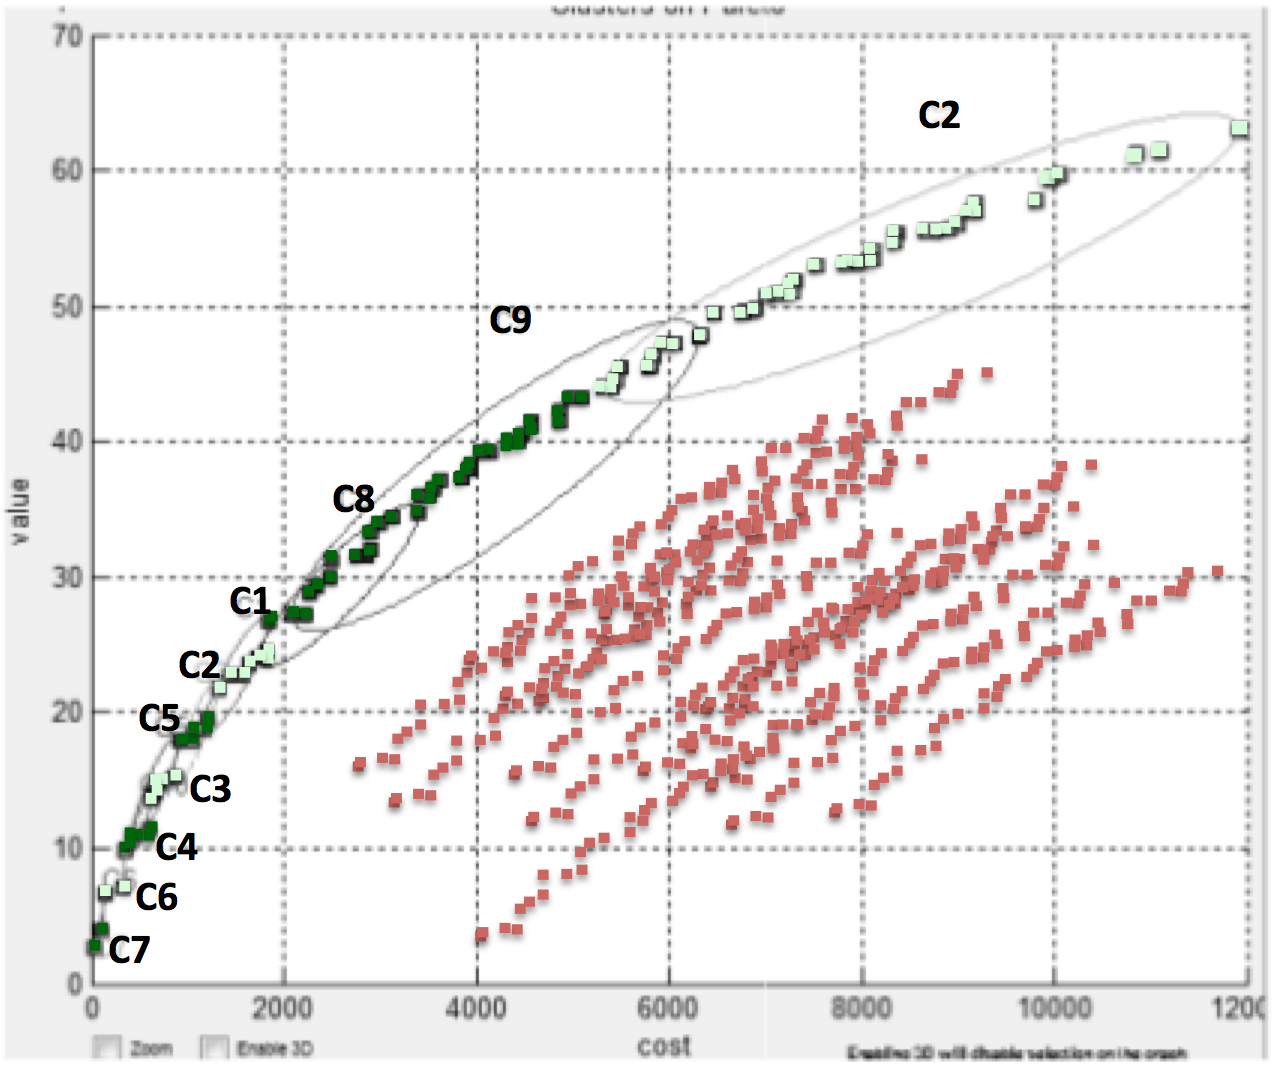
\includegraphics[width=3in]{figures/amus.png}
\caption{Exploring options for configuring London
Ambulances~\cite{veer11} (to minimize $X$ and maximize $Y$).
 An SBSE
has rejected thousands of options (shown in red) 
to isolate clusters of better solutions C1,C2,etc (shown in green). }\label{fig:one}
\end{figure}

One standard method to reduce the space of solutions is to find the {\em Pareto frontier}; i.e.
the subset of solutions 
that are not worse than any other (across all goals)
but better on at least one goal. 
For example,
the green dots
in \fig{one} are an example of such a Pareto
frontier (and the red dots are called the {\em dominated} examples).

The problem here is that even the Pareto frontier can be too large to understand.
Harman cautions that many frontiers are very {\em crowded}; i.e. contain thousands (or more)
candidate solutions~\cite{harm13}.
Hence, researchers like  Verrappa and Leiter add post-processors to SBSE
tools that (a)~cluster the Pareto frontier (like in~\fig{one};  C1,C2,etc);
then (b)~show users a small number of examples per cluster. 
That approach has two issues. Firstly, it can lose some information;
e.g. clusters C2 and C9 in \fig{one} are much larger
than the others. 
Secondly, it requires the SBSE tool to terminate
before the users can get any explanation---which is a
problem for very slow computations.  Zuluaga et
al. comment on the cost of SBSE for
software/hardware co-design: ``synthesis of only one
design can take hours or even
days.''~\cite{Zuluaga:13}.  Harman~\cite{harm13}
comments on the problems of evolving a test suite
for software if every candidate solution requires a
time-consuming execution of the entire system. Such
test suite generation can take weeks of execution
time. For such very slow computational problems, it
would be useful to obtain some initial results that
(say) allow users to guide the rest of the
computation.

This paper introduces GALE, an SBSE tool that addresses
the above issues.
GALE is an evolutionary learner
where solutions in the next generation
are mutations of the previous generation.
To avoid very large clusters (such as those seen in \fig{one}),
GALE generates many small
clusters. Using  a linear-time recursive
descent algorithm, GALE splits solutions into two
equal-size halves. It then recurses on each half,
stopping when {\em leaf} splits have less than   $\sqrt{N}$
items.

To optimize very long computations, at each level of
recursion,  GALE 
evaluates only the two most different (i.e. most distant)
solutions.  We call
these solutions the {\em poles}.
During recursion, if one pole dominates
the other, GALE skips the dominated half.
GALE's leaf clusters contain solutions
that dominate the skipped solutions; i.e.
they
are candidates for the Pareto frontier.
GALE contributes to the next generation by mutating solutions
in each leaf  away from the worst pole in that leaf.

Note that GALE is different than the approach
of Veerappa \& Letier.
GALE does not use clustering as a post-process to some SBSE tool.
Rather, GALE {\em replaces} the need for a post-processor with its tool called WHERE, which explores only two evaluations per recursive split
of the data. Hence, this algorithm
performs at most $2{\log_2}(N)$ evaluations per
generation (and less when recursion ignores
dominated solutions). 

This paper assesses the value of GALE for SBSE.
Within that assessment, there are two fundamental issues.
Firstly,  concerning  the  number  of  evaluations compared  to  that  of  other  algorithms:
\begin{quote}
{\bf RQ1 (speed):} Does GALE terminate faster than other SBSE tools?
\end{quote}
This is a concern since GALE's recursive approach means that, apart from optimization,
GALE must also cluster all the current solutions.
Theoretically, this could mean that   GALE is  slower than other SBSE tools.

The second fundamental issue  
concerns  the  quality  of  the  results  returned by GALE:
\begin{quote}
{\bf RQ2 (quality):} Does GALE return similar or better
solutions than other SBSE tools?
\end{quote}
This is a concern since GALE only examines $\log(N)$ of the solutions.
Theoretically, this could mean that GALE misses  optimizations
 found by other tools.



\subsection{Structure of this Paper}
This paper presents evidence that GALE's rapid exploration of the solution space
is useful and effective.
After some notes on related work (in Section 2)
we discuss the internal details of GALE (in Section 3). 
The algorithm is then tested on a range of models of varying sizes, using
a range of models described in Section 4.
Section~5 presents our results.
As to {\bf RQ1 (speed)}, GALE ran much faster than
other SBSE tools, especially for very large models.
For example, 
for our largest model, GALE terminated in four minutes
while other tools needed seven hours.
As to {\bf RQ2 (quality)}, we found that the 
solutions generated by GALE were rarely worse than other tools (and sometimes,
they were much better). 


\subsection{Availability}

GALE is released under the GNU Lesser GPL. 
It is available as part of the JMOO package (Joe's multi-objective optimization), which
incorporates DEAP (Distributed Evolutionary Algorithms in Python~\cite{jmlr12}).
GALE is available for  download 
from~\url{http://unbox.org/open/tags/JMOO}.

%% Lastly, even when humans are not in the loop for reasoning about a model, it is important for search-based
%% SE to reduce the number of evaluations required for controlling a model. As software systems grow ever larger
%% and more complex, it becomes harder to explore all their internal effects. Hence, tools like GALE are required
%% to map out and better understand  the shape of those internal effects.







\section{Related Work}
This section explains the following terms.
GALE is an {\em active learner} that implements a {\em multi-objective evolutionary algorithm} (MOEA).
MOEAs are frequently used for {\em search-based software engineering} (SBSE).
GALE's mutators use  {\em continuous domination} and {\em spectral learning}
to push solutions away from worse regions.

\subsection{SBSE}


In software engineering (SE), it is often necessary to trade
off between many competing objectives.  This task is often handled
by search-based software engineering (SBSE) tools.
For example, Rodriguez et
al.~\cite{rod11} used a systems model of a software project~\cite{deb00afast}
 to search for inputs that generate favorable outputs---in this case, outputs that
most decrease time and cost while increasing productivity. That study
generated a three-dimensional surface model where managers could explore
trade-offs between the objectives of cost, time and productivity.  In other
work, Heaven \& Letier~\cite{heaven11} studied a quantitative
goal graph model of the requirements of the London Ambulance
Services. The upper layers of that requirements model were a standard
Van Lamsweerde goal graph~\cite{lam00}, while the leaves drew their
values from statistical distributions. Using that model, they found
decisions that balance speed \& accuracy of ambulance-allocation
decisions. Subsequent work by Veerappa \& Letier (discussed in the introduction)
explored methods to better explain the generated set of solutions~\cite{veer11}.
For a list of other SBSE applications, see \fig{tasks}.

Due to the complexity
of these tasks, exact optimization methods may be impractical.
Hence, researchers often resort to various meta-heuristic  approaches.
In the 1950s, when
computer RAM was very small, a standard technique was simulated
annealing (SA)~\cite{kirkpatrick83}. SA generates {\em new} solutions
by randomly perturbing (a.k.a. ``mutating'') some part of an {\em old}
solution.  {\em New} replaces {\em old} if (a) it scores higher; or
(b) it reaches some probability set by a ``temperature'' constant. Initially,
temperature is high so SA jumps to sub-optimal solutions (this allows
the algorithm to escape from local minima). Subsequently, the
``temperature'' cools and SA only ever moves to better {\em new}
solutions.
SA is often used in SBSE
e.g.~\cite{fea02a,me07f,me07g}, perhaps due to its simplicity.

In the 1960s, when more RAM became available, it became standard to
generate many {\em new} mutants, and then combine together parts of
promising solutions~\cite{goldberg79}.  Such {\em evolutionary
  algorithms} (EA) work in {\em generations} over a population of
candidate solutions.  Initially, the population is created at random.
Subsequently, each generation makes use of select+crossover+mutate
operators to pick promising solutions, mix them up in some way, and
then slightly adjust them.
EAs are also often used in SBSE, particularly in test case generation; e.g.~\cite{andrews07,andrews10}.

Later work focused on creative ways to control the
mutation process. Tabu search and scatter search
work to bias new mutations away from prior
mutations~\cite{Glover1986563,Beausoleil2006426,Molina05sspmo:a,4455350}.
Differential evolution mutates solutions by
interpolating between members of the current
population~\cite{storn97}.  Particle swarm
optimization randomly mutates multiple solutions
(which are called ``particles''), but biases those
mutations towards the best solution seen by one
particle and/or by the neighborhood around that
particle~\cite{pan08}.
These methods are often used for parameter tuning for other learners.
For example, Cora et al.~\cite{cora10} use tabu search to learn the parameters
of a radial bias support vector machine for learning effort estimation models.

\begin{figure}[!t]
\small
\begin{tabular}{|p{3.1in}|}\hline
\bi
\item
{\em  Next release planning:}
Deliver most functionality
in least time and cost~\cite{zhang07a,bagnall01,DurilloZAHN11}.
\item {\em Risk management:} Maximize the covered requirements while minimizing the
cost of  mitigations applied  (to avoid possible problems)~\cite{fea02a,feather03,me08b}.
\item {\em Explore high-level designs:} Use most features
avoiding defects, with  least development time,  avoiding violations of
constraints~\cite{sayyad13a,sayyad13b}.
\item {\em Improve low-level designs:}
Apply automatic refactoring tools to object-oriented design in order improve the internal
cohesiveness of that design~\cite{ocinneide12}.
\item
{\em  Test case generation:} Adjust  test suites
to increase program  coverage by those tests~\cite{andrews07,andrews10,me09m}.
\item
{\em Regression tests:} Find tests that run fastest, with the most odds of being relevant
to  recently changed code, with the greatest probability of failing~\cite{weimer13}.
\item
{\em Cloud computing:}
For distributed CPUs and disks, adjust allocation and assignment of tasks
to  trade-off between availability,
performance and cost~\cite{harman13}.
\item
{\em Predictive Modeling:} Tune  data miner's parameters to improve  predictions of
software cost~\cite{cora10}.
\ei\\\hline
\end{tabular}
\caption{Some optimization tasks explored by SBSE.}\label{fig:tasks}
\end{figure}

\subsection{MOEA}

This century, there has been much new work on
multi-objective evolutionary algorithms (MOEA) with 2 or 3 objectives
(as
well as many-objective optimization, with many more
objectives).  Multi-objective evolutionary algorithms
such as NSGA-II~\cite{deb00afast},
SPEA2~\cite{zit02}, or IBEA~\cite{Zitzler04indicator-basedselection}, try to push
a cloud of solutions towards an outer envelope of
preferred solutions.
These MOEAs eschew the idea of
single solutions, preferring instead to map the
terrain of all useful solutions.  For example, White
et al.~\cite{white09} use feature attributes related
to resource consumption, cost and appropriateness of
the system. Similarly, Ouni et al. are currently
working on an extension to their recent ASE journal
paper~\cite{ouni13} where they use MOEAs
 to reduce software defects and maintenance cost
via code refactoring (members of that team now explore a
15 objective problem).


\subsection{MOEA \& Domination}\label{sec:cdom}

MOEA tools
use a
{\em  domination function} to find
promising solutions for use in the next generation.
{\em Binary domination} says that solution $x$ ``dominates''
solution $y$ if solution $x$'s objectives are never worse than  solution $y$
and at least one objective in solution $x$ is better than its counterpart in $y$; i.e.
 $\left\{ \forall o  \in \textit{objectives}\;\mid\; \neg ( x_o \prec y_o )\right\}$
and
 $\left\{
\exists o \in \text{objectives} \;\mid\; x_o \succ y_o\right\}$, where ($\prec,\succ$) tests if $x_o$ is (worse,better) than $y_o$.
 Recently, Sayyad~\cite{sayyad13a} studied binary domination for SBSE
with 2,3,4 or 5 objectives.  Binary domination performed as well as anything else
for 2-objective problems but very few good solutions were found for
the 3,4,5-goal problems.  The reason was simple: binary domination  only returns
{\em \{true,false\}}, no matter the difference between $x_1,x_2$. As the objective
space gets more divided at higher dimensionality, a more nuanced approach is required.


While binary domination just returns (true,false), a {\em continuous domination} function sums
the total improvement of solution $x$ over all other solutions~\cite{Zitzler04indicator-basedselection}.
In the IBEA genetic algorithm~\cite{Zitzler04indicator-basedselection}, continuous domination is defined as the sum of the
differences between objectives (here ``$o$'' denotes the number of objectives),
raised to some exponential power.
Continuous domination favors $y$ over $x$ if $x$ ``losses'' least:

\begin{equation}\label{eq:cdom}
\begin{array}{rcl}
\textit{worse}(x,y)& =& \textit{loss}(x,y) > \textit{loss}(y,x)\\
\textit{loss}(x,y)& = &\sum_j^o -e^{w_j(x_j - y_j)/o	} / o
\end{array}
\end{equation}
In the above, $w_j\in \{-1,1\}$, depending on whether
we seek to maximize goal $x_J$.   
To prevent issues with exponential functions,
the objectives are normalized.



When the domination function is applied to a
population it can be used to generate the {\em
  Pareto frontier}, i.e.  the space of non-dominated
and, hence, most-preferred solutions. A standard
MOEA strategy is to generate new individuals, then
focus just on those on the Pareto
frontier. Different MOEA algorithms find this
frontier in different ways.  For example, GALE's method
was outlined in the introduction.
On the other hand, SPEA2
favors solutions that dominate the most number of
other solutions that are not nearby (and, to break
ties, it uses a density estimation technique).  Further,
NSGA-II uses a non-dominating sort
procedure to divide the solutions into {\em bands}
where {\em band}$_i$ dominates all of the solutions
in {\em band}$_{j>i}$ (and NSGA-II favors the
least-crowded solutions in the better bands).
Finally, IBEA uses continuous dominance to find the
solutions that dominate all others.


\lstset{
    language=Python,
    basicstyle=\ttfamily\fontsize{2.7mm}{0.8em}\selectfont,
    breaklines=true,
    prebreak=\raisebox{0ex}[0ex][0ex]{\ensuremath{\hookleftarrow}},
    frame=l,
    showtabs=false,
    showspaces=false,
    showstringspaces=false,
    keywordstyle=\bfseries,
    emph={furthest,gale,better,improved,where,fastmap,split,project,mutate,mutate1}, emphstyle=\bfseries\color{blue},
    stringstyle=\color{green!50!black},
    commentstyle=\color{gray}\itshape,
    numbers=left,
    captionpos=t,
    escapeinside={\%*}{*)}
}
\begin{figure}[!b]
\begin{lstlisting}[mathescape,frame=l,numbers=left]
def fastmap(data): 
  "Project data on a line between 2 distant points"
  z          = random.choose(data)
  east       = furthest(z, data)
  west       = furthest(east, data)
  data.poles = (west,east)
  c          = dist(west,east)     
  for one in data.members: 
    one.pos = project(west,east,c,one)
  data = sorted(data) # sorted by 'pos'
  return split(data)

def project(west, east, c, x): 
  "Project x onto line east to west"
  a = dist(x,west)
  b = dist(x,east)
  return (a*a + c*c - b*b)/(2*c) # cosine rule

def furthest(x,data): # what is furthest from x?
  out, max = x,0
  for y in data:
    d = dist(x,y)
    if d > max: out, max = y, d
  return out

def split(data): # Split at median
   mid = len(data)/2; 
  return data[mid:], data[:mid]
\end{lstlisting}

\caption{Splitting data with FastMap}
\label{fig:fastmapCode}   
\end{figure}
\subsection{Active Learning}

Active learners make conclusions by asking for {\em
more} information on the {\em least} number of
items.  For optimization,  such active learners
reflect over a population of decisions and only
compute the objective scores for a small, {\em most
informative subset} of that
population~\cite{Zuluaga:13}.  

For example, Zuluaga et
al.~\cite{Zuluaga:13} use a {\em response surface
  method} for their MOEA active learner.  Using some
quickly-gathered information, they build an
approximation to the local Pareto frontier using a
set of Gaussian surface models. These models allow
for an extrapolation between known members of the
population.  Using these models, they can then
generate approximations to the objective scores of
mutants. Note that this approach means that (say)
after 100 evaluations, it becomes possible to
quickly approximate the results of (say) 1000 more.

GALE's active learner finds its {\em most information subset} via the WHERE
clustering procedure. As discussed in the next section,
WHERE recursively divides the candidates into many small clusters,
then looks for two most different (i.e. most distant) points
in each cluster. For each cluster, GALE then evaluates only these
two points. 







\begin{figure}[!t]
{\fontsize{2mm}{0em}\selectfont 
~~~~~~~~\begin{minipage}[t]{1.5in}
{\small 
{\bf Figure4a:} 
Dividing 400 instances using just the independent variables.}

\begin{verbatim}
400
|  > 200
|  |  > 100
|  |  |  > 50
|  |  |  |  > 25
|  |  |  |  < 25
|  |  |  < 50
|  |  |  |  > 25
|  |  |  |  < 25
|  |  < 100
|  |  |  > 50
|  |  |  |  > 25
|  |  |  |  < 25
|  |  |  < 50
|  |  |  |  > 25
|  |  |  |  < 25
|  < 200
|  |  > 100
|  |  |  > 50
|  |  |  |  > 25
|  |  |  |  < 25
|  |  |  < 50
|  |  |  |  > 25
|  |  |  |  < 25
|  |  < 100
|  |  |  > 50
|  |  |  |  > 25
|  |  |  |  < 25
|  |  |  < 50
|  |  |  |  > 25
|  |  |  |  < 25
\end{verbatim}
\end{minipage}~~~~~~~~~\begin{minipage}[t]{1.5in}
{\small
{\bf Figure4b}: Dominated sub-trees are pruned via active learning techniques(~\tion{al}).}

\begin{verbatim}
400           
|  > 200  <-- pruned
|  < 200 
|  |  > 100 
|  |  |  > 50 <-- pruned
|  |  |  < 50 
|  |  |  |  > 25 <-- pruned
|  |  |  |  < 25 
|  |  < 100 
|  |  |  > 50 
|  |  |  |  > 25 
|  |  |  |  < 25 
|  |  |  < 50 
|  |  |  |  > 25 
|  |  |  |  < 25 
\end{verbatim}
\end{minipage}}
\caption{Recursive division via WHERE of 400 instances 
(using FastMap).}\label{fig:cluster1}
\end{figure}
 


\subsection{Fast Spectral Learning}
WHERE is a {\em spectral learner}~\cite{KamvarKM03}; i.e. given solutions with $d$ possible decisions,
it
re-expresses those $d$ dimensions in terms of the
$e$ eigenvectors of that data.
This speeds up the reasoning since we then only need to
explore the $e<d$ dimensions of the eigenvectors.

A widely-used spectral learner is a principal
 component analysis (PCA).  For example, PDDP ({\em
 Principal Direction Divisive
 Partitioning})~\cite{boley98} recursively
 partitions data according to the median point of
 data projected onto the first PCA component of the
 current partition.

WHERE~\cite{me12d} is a linear time variant of PDDP  which uses the FastMap heuristic~\cite{Faloutsos1995}
to quickly find the first component.
Platt~\cite{platt05} shows that FastMap belongs to the Nystr\"om family
of algorithms that find approximations to eigenvectors.

The FastMap heuristic (shown in \fig{fastmapCode})
projects all data onto a line
connecting the two distant points found on lines 3-5\footnote{
To define distance, WHERE uses 
the standard Euclidean distance method proposed by 
Aha et al.~\cite{aha91}; that is:
$dist(x,y)= \sqrt{\sum_{i\in d} (x_i - y_i)^2}/\sqrt{ 
\left\vert{d}\right\vert }$ where distance is
computed on the independent decisions $d$ of each candidate solution;
all $d_i$ values are normalized min..max, 0..1; and the calculated distance normalized by dividing by the maximum distance
across the $d$ dimensions.}. 
FastMap finds these two distant points in near-linear
time. The search for the poles needs only
$O(N)$ distance comparisons (lines 19 to 24).
The slowest part of this search is the sort used to find the median $x$ value 
(line 10) but even that
can be reduced to  asymptotically optimal linear-time
via the standard median-selection algorithm~\cite{hoare61}.

This FastMap procedure returns the data split into two
equal halves.
WHERE recurses on the two halves found by FastMap,
terminating when some split
has less than $\sqrt{N}$ items.
For example, consider 400 cars described in terms of
their {\em independent} variables
(such as number of cylinders, engine displacement, etc)
as well as their {\em dependent} variables such as
acceleration and miles per gallon (mpg).
Using the independent variables,
WHERE would recursively divide that data as per Figure~4a to generate 16 leaf
clusters, each of which contains 25 cars.



\begin{figure}[!b]
\begin{lstlisting}[mathescape,frame=l,numbers=left]
def where(data, scores={}, lvl=10000, prune=True):  
  "Recursively split data into 2 equal sizes."
  if lvl < 1: 
     return data # stop if out of levels
  leafs      = [] # Empty Set
  left,right = fastmap(data)
  west, east = data.poles
  $\omega=\sqrt{\mu}$ # enough data for recursion
  goWest = len(left) > $\omega$  
  goEast = len(right) > $\omega$ 
  if prune: # if not pruning, ignore this step
    if goEast and better(west,east,scores): 
       goEast = False 
    if goWest and better(east,west,scores): 
       goWest = False 
  if goWest:  
     leafs += where(left,  lvl - 1, prune)  
  if goEast:  
     leafs += where(right, lvl - 1, prune) 
  return leafs

def better(x,y,scores):
   "Check if not worse(y,x) using $\eq{cdom}$. If any"
   "new evaluations, cache them  in 'scores'."
\end{lstlisting}

\caption{Active learning in GALE:
recursive division of the data;
only evaluate two distant points in each cluster;
only recurse into non-dominated halves.
In this code, $\mu$ is size of the original data set.
}
\label{fig:whereCode}   
\end{figure}




\section{Inside GALE}
The  {\em \underline{g}eometric}, {\em \underline{a}ctive \underline{le}arner} called 
GALE interfaces to models using the following functions:
\bi
\item Models create candidates, each  with $d$ decisions. 
\item $\mathit{lo}(i), \mathit{hi}(i)$ report the minimum and maximum
legal values for decision $i\in d$.
\item $\mathit{valid}(\mathit{candidate})$ 
checks if the decisions
do not violate any domain-specific constraints.
\item  From the decisions,
a model can compute $o$  objective scores (used in \eq{cdom}).
\item $\mathit{minimizing}(j)$ returns true,false if the goal
is to minimize,maximize (respectively) objective $j \in o$.
\ei
%% GALE explores the candidates via a combination of optimization and data
%% mining. Given a current population of candidates, the
%% algorithm learns a decision tree whose leaves are non-dominated
%% candidates. These leaves are the seeds for the next generation 
%% of candidates.




\subsection{Active Learning and GALE}\label{sec:al}
GALE's active learner, shown in \fig{whereCode}, is a
variant to the WHERE spectral
learner discussed above.
To understand this procedure, recall 
that WHERE splits the data
into smaller
 clusters, each of which is characterized by two
distant points called {\em west,east}. In that space,
{\em left} and {\em right} are  50\% of the
data, projected onto a line running {\em west} to {\em east},
 split at the median.
When exploring $\mu$ candidates, recursion
halts at splits smaller
than $\omega=\sqrt{\mu}$.


GALE's active learner assumes that it
only needs to evaluate
the 
{\em most informative subset} 
consisting of the {\em poles} used to
recursively divide the data. 
Using \eq{cdom}, GALE checks for domination between
the poles and only recurses into any non-dominated halves.
This process, shown in \fig{whereCode}, uses FastMap
to split the data. 
In that \fig{whereCode}, 
 lines 12 and 14 show the domination
pruning that disables recursion into any dominated half.



Figure~4b demonstrates this pruning.
Our 400 cars are divided in same way as Figure~4a---but
pruning sub-trees with a dominated pole (here
we assume that we want cars that have maximal acceleration and miles per gallon).
For this data (http://goo.gl/VpU8Qd), GALE's active learner
pruned
275 solutions, leaving 
 five leafs of non-dominated solutions.


Given GALE's recursive binary division of $\mu$ solutions, and that this
 domination tests only two
solutions in each division, then GALE
performs  a maximum of $2log_2(\mu)$ evaluations. When GALE prunes sub-trees,
the actual number of evaluations is less than this maximum; e.g. Figure 4b was generated
after checking the dependent variables of just 14 instances (out of 400).



\begin{figure}[!b]
\begin{lstlisting}[mathescape,frame=r,numbers=right]
def mutate(leafs, scores): 
  "Mutate all candidates in all leafs."
  out = [] # Empty Set
  for leaf in leafs:
    west,east = leafs.poles
    if better(west,east, scores): # uses \eq{cdom}
       east,west = west,east # east is the best pole
    c = dist(east,west)
    for candidate in leaf.members:
      out += [mutate1(candidate, c, east, west)]
  return out 

def mutate1(old,c,east,west,$\gamma$=1.5): 
  "Nudge the old towards east, but not too far."
  tooFar = $\gamma$ * abs(c)
  new    = copy(old)
  for i in range(len(old)):
    d = east[i] - west[i]
    if not d == 0: #there is a gap east to west
      d  = -1 if d < 0 else 1 #d is the  direction
      x  = new[i]* (1 + abs(c)*d) # nudge along d 
      new[i]= max(min(hi(i),x),lo(i))#keep in range
  newDistance = project(west,east,c,new) -
                project(west,east,c,west)
  if abs(newDistance) < tooFar and valid(new): 
        return new
  else: return old
\end{lstlisting}

\caption{Mutation with GALE.
By line 7, GALE has determined that the {\em east}
pole is preferred  to {\em west}.
At line 23,24, the {\tt project}
function of \fig{fastmapCode}  is used
to check 
we are not rashly mutating a candidate too far away from
the region that originally contained it.}
\label{fig:mutantCode}   
\end{figure}
\subsection{Geometry-based Mutation}
GALE's mutation policy is shown in \fig{mutantCode}.
Most MOEAs build their next generation of solutions
by a {\em random mutation} of members of the last
generation. GALE's mutation policy is somewhat
different in that it is a {\em directed mutation}.
Specifically, GALE reflects on the geometry of the
solution space, and mutates instances along
gradients within that geometry. 
To inspect that geometry, GALE reflects over the poles
in each leaf cluster. In the case where one pole
is {\em better} than another, it makes sense to
nudge all solutions in that cluster away from the
worse pole and towards the better pole.  



By nudging solutions along a line
running from {\em west} to {\em east}, we are
exploiting spectral learning to implement a {\em
spectral mutator}; i.e. one that works across a
dimension of greatest variance that is synthesized
from the raw dimensions.  That is, GALE models the
local Pareto frontier as many linear models
drawn from the local eigenvectors of different
regions of the solution space.  Note that we prefer
GALE's approach to the Gaussian process models used
by Zuluaga et al.~\cite{Zuluaga:13} since, with GALE, we have
guarantees of linear-time execution.



\begin{figure}[!t]
\begin{lstlisting}[mathescape,frame=l,numbers=left]
def gale(enough=16,  max=1000,  $\lambda=3$):
  "Optimization via Geometric active learning"
  pop      = candidates($\mu$) # the initial population
  patience = $\lambda$
  for generation in range(max):
    # mutates candidates in non-dominated leafs
    scores  = {} # a cache for the objective scores 
    leafs   = where(pop, scores)
    mutants = mutate(leafs, scores)
    if generation > 0:  
      if not improved(oldScores ,scores):
        patience = patience - 1 #losing  patience
      oldScores = scores #needed for next generation
      if patience < 0: #return enough candidates
        leafs=where(pop,{},log2(enough),prune=False)
        return [ y.poles for y in leafs ] 
    #build up pop for next generation
    pop = mutants + candidates($\mu$-len(mutants))   

def improved(old,new):
  "Report some success if any improvement."
  for j in range(len(old)):
    before = # old mean of the j-th objective
    now    = # new mean of the j-th objective
    if minimizing(j):
      if now < before: return True
    elif now > before: return True
  return False 
\end{lstlisting}

\caption{GALE's top-level driver.}
\label{fig:galeCode}   
\end{figure}




\subsection{Top-level Control}

\fig{galeCode} shows GALE's top-level controller.  As seen in that figure, 
the algorithm  is an
evolutionary learner which iteratively builds,
mutates, and prunes a population of size $\mu$
using the active
learning version of WHERE.
The {\em candidates} function (at line 3 and 18) adds random items to the 
population. The first call to this function (at line 3)
adds $\mu$ new items. The subsequent call (at line 18) rebuilds the population back up to $\mu$ after
WHERE has pruned solutions in dominated clusters.

Also shown in that figure is GALE's termination
procedure: GALE exits after $\lambda$ generations with no improvement
in any goal.
Note that, on termination, GALE calls WHERE one last
time at line 15 to find {\em enough} examples to
show the user. In this call, domination pruning is
disabled, so this call returns the poles of the
leaf clusters.











\section{Assessing GALE}

\subsection{Comparison Algorithms}
According to the recent 2013 literature survey by Sayyad and Ammar~\cite{sayyad13c}, 
NSGA-II and SPEA2 are the two most widely-used SBSE tools.
Hence, these will be used to comparatively evaluate GALE.

To provide a reusable experimental framework, we
implemented GALE as part of a Python software
package called JMOO (Joe's Multi-Objective
Optimization).  JMOO allows for
testing experiments with different MOEAs and
different MOPs (multi-objective problems), and
provides an easy environment for the addition of
other MOEAs.  
JMOO uses the DEAP
toolkit~\cite{jmlr12} for its
implementations of  NSGA-II and SPEA2.

To provide a valid base of comparison, we applied
the same parameter choices across all
experiments:
\bi
\item
MOEAs use the same
population$_0$ of size $\mu=100$.
\item All MOEAs had the same early
stop criteria (see the
$\lambda=3$ test of \fig{galeCode}).
Without early stop, 
number of generations is set at {\em max}$=20$.
\ei

NSGA-II and SPEA2 require certain
 parameters for crossover and
mutation. We used the default parameters from the DEAP
package:
\bi
\item A crossover frequency of  $cx=0.9$;
\item The mutation rate is $mx=0.1$, and $eta=1.0$ determines how often
mutation occurs and how similar mutants are to their
parents (higher $eta$ means more similar to the
parent).
\ei
\subsection{Models Used in This Study}
\subsubsection{Benchmark MOEA Models}
This paper applies GALE, NSGA-II and SPEA2 to various models.
The first  set of models are the standard benchmark
 models used by the MOEA
community to assess new algorithms.
For details on these models (called Golinski, Osyczka2, Schaffer,
Srinivas, Tanaka, Viennet2, and ZDT1), see \fig{nocon} and \fig{con}.


\begin{figure*}\footnotesize
	\centering
		\begin{tabular}{ | l | c | l | c | }
		\hline
%		\multicolumn{4}{ | c | }{Unconstrained Multi-Objective Functions}\\		\hline
		Name & n & Objectives & Variable Bounds\\\hline\hline
		Schaffer & 1 & \begin{tabular}{ l }
		$ f_1(x) = x^2 $\\
		$ f_2(x) = (x-2)^2 $
		\end{tabular} & {$ -10 <= x <= 10 $}\\\hline

		Viennet 2 & 2 & \begin{tabular}{ l }
		{$ f_1(\vec{x})= \frac{(x_1-2)(x_1-2)}{2} + \frac{(x_1+1)(x_1+1)}{13} + 3 $}\\
		{$ f_2(\vec{x})= \frac{(x_1+x_2-3)(x_1+x_2-3)}{36} + \frac{(-x_1+x_2+2)(-x_1+x_2+2)}{8} - 17 $}\\
		{$ f_3(\vec{x})= \frac{(x_1+2x_2-1)(x_1+2x_2-1)}{175} + \frac{(2x_2-x_1)(2x_2-x_1)}{17} - 13 $}
		\end{tabular} & {$ -4 <= x_i <= 4 $}\\
		\hline

		ZDT1 & 30 & \begin{tabular}{ l }
		{$ f_1(\vec{x})= x_1 $}\\
		{$ f_2(\vec{x})=  g * (1 - \sqrt{\frac{x_1}{g}})$}\\
		{$ g(\vec{x}) = 1 + \frac{9}{n-1}\sum_{i=2}^{n}(x_i) $}
		\end{tabular} & {$ 0 <= x_i <= 1 $}\\
		\hline

		Golinksi & 7 & \begin{tabular}{ l }
		{$ A(\vec{x}) = 0.7854 x_1 x_2^2 (\frac{10 x_3^2}{3.0} + 14.933 x_3 - 43.0934) $}\\
		{$ B(\vec{x}) = -1.508 x_1 (x_6^2 + x_7^2)+7.477(x_6^3 + x_7^3) + 0.7854(x_4*x_6^2 + x_5*x_7^2) $}\\
		{$ aux(\vec{x}) = 745.0 \frac{x_4}{x_2 * x_3} $}\\
		{$ f_1(\vec{x})= A + B $}\\
		{$ f_2(\vec{x})= \frac{\sqrt{aux^2 + 1.69e7}}{0.1 x_6^3} $}
		\end{tabular} & \begin{tabular}{ c }
		{$ 2.6 <= x_1 <= 3.6 $}\\
		{$ 0.7 <= x_2 <= 0.8 $}\\
		{$ 17.0 <= x_3 <= 28.0 $}\\
		{$ 7.3 <= x_4, x_5 <= 8.3 $}\\
		{$ 2.9 <= x_6 <= 3.9 $}\\
		{$ 5.0 <= x_7 <= 5.5 $} 
		\end{tabular}
		\\ \hline



		\end{tabular}
		\caption{Unconstrained standard MOEA benchmark problems. Note: all objectives
are to be minimized.}
	\label{fig:nocon}
\end{figure*}
\begin{figure*}\footnotesize
	\centering
		\begin{tabular}{ | l@{~} | l@{~} | l@{~} | l@{~} | c@{~} | }
			\hline
%			\multicolumn{5}{ | c | }{Constrained Multi-Objective Functions}\\\hline
			Name & n & Objectives & Constraints & Variable Bounds\\\hline \hline	

			Srinivas & 2 & \begin{tabular}{ l }
				{$ f_1(\vec{x}) = (x_1 - 2)^2 + (x_2-1)^2 + 2 $}\\
				{$ f_2(\vec{x}) = 9x_1 - (x_2 -1)^2 $}\end{tabular} & \begin{tabular}{ l }
				{$ g_1(\vec{x}) = x_2 + 9x_1 >= 6 $}\\
				{$ g_2(\vec{x}) = -x_2 + 9x_1 >= 1 $}\end{tabular} & {$ -20 <= x <= 20 $}\\\hline

			Tanaka & 2 & \begin{tabular}{ l }
				{$ f_1(\vec{x}) = x_1 $}\\
				{$ f_2(\vec{x}) = x_2 $}\end{tabular} & \begin{tabular}{ l }
				{$ A(\vec{x}) = 0.1 \cos{(16\arctan{(\frac{x_1}{x_2})})} $}\\
				{$ g_1(\vec{x}) = 1 - x_1^2 - x_2^2 + A <= 0 $}\\
				{$ g_2(\vec{x}) = (x_1 - 0.5)^2 + (x_2 - 0.5)^2 <= 0.5 $}\end{tabular} & {$ -\pi <= x <= \pi $}\\\hline

			Osyczka 2 & 6 & \begin{tabular}{ l }
				{$ A(\vec{x}) = 25 (x_1 - 2)^2 + (x_2 - 2)^2 $}\\
				{$ B(\vec{x}) =  (x_3 - 1)^2*(x_4 - 4)^2 + (x_5 - 2)^2$}\\
				{$ f_1(\vec{x}) =  0 - A - B  $}\\
				{$ f_2(\vec{x}) = x_1^2 + x_2^2 + x_3^2 + x_4^2 + x_5^2 + x_6^2 $}
				\end{tabular} & \begin{tabular}{ l }
				{$ g_1(\vec{x}) = x_1 + x_2 - 2 >= 0 $}\\
				{$ g_2(\vec{x}) = 6 - x_1 - x_2 >= 0 $}\\
				{$ g_3(\vec{x}) = 2 - x_2 + x_1 >= 0 $}\\
				{$ g_4(\vec{x}) = 2 - x_1 + 3 x_2 >= 0 $}\\
				{$ g_5(\vec{x}) = 4 - (x_3-3)^2 - x_4 >= 0 $}\\
				{$ g_6(\vec{x}) = (x_5-3)^3 + x_6 - 4 >= 0$}
				\end{tabular} & \begin{tabular}{ c }
					{$ 0 <= x_1,x_2,x_6 <= 10 $}\\
					{$ 1 <= x_3,x_4 <= 5 $}\\
					{$ 0 <= x_5 <= 6 $}
		\end{tabular}
		\\ \hline
		\end{tabular}
		
		\caption{Constrained standard benchmark MOEA problems. Note: all objectives
are to be  minimized.}\label{fig:con}
\end{figure*}


\begin{figure*}%[!t]
\scriptsize
    \centering
    \begin{tabular}{|l|l|p{4in}|c|}
        \hline
        Short name &Decision             & Description         &Controllable                                        \\ \hline
        Cult&Culture              & Number (\%) of requirements that change. & yes \\\hline
        Crit&Criticality           & Requirements cost effect for safety critical systems  (see \eq{cmcrit} in the appendix). & yes\\\hline
        Crit.Mod&Criticality Modifier & Number of (\%) teams affected by criticality   (see \eq{cmcrit} in the appendix).   & yes           \\ \hline
        Init. Kn&Initial Known        & Number of (\%) initially known requirements.             & no     \\ \hline
        Inter-D&Inter-Dependency     & Number of (\%) requirements that have interdependencies.  Note that dependencies are requirements within
the {\em same} tree (of requirements), but interdependencies are requirements that live in {\em different} trees.   & no            \\\hline
        Dyna&Dynamism             & Rate of how often new requirements are made (see \eq{dymn} in the appendix). & yes                    \\ \hline
        Size&Size            & Number of base requirements in the project.& no \\        \hline
        Plan&Plan                 & Prioritization Strategy (of requirements): one of
        0= Cost Ascending;  1= Cost Descending; 2= Value Ascending; 3= Value Descending;
        4 = $\frac{Cost}{Value}$ Ascending.
%Note that a standard agile strategies use ``Value Descending'', i.e. plan=3~\cite{me09j}.
 & yes \\\hline
     T.Size&Team Size            & Number of personnel in each team   & yes                         \\ 
        \hline
    \end{tabular}
    \caption {List of Decisions used in POM3. 
The optimization task is to find settings for the controllables in the last column.
}\label{fig:pom3decisions}
\end{figure*}
\begin{figure*}%[!t]
\footnotesize
\begin{center}
    \begin{tabular}{r|p{1.5in}|p{1.5in}|p{1.5in}}
                     & POM3a                         & POM3b             &POM3c       \\ 
                             & A broad space of projects. & Highly critical small projects& Highly dynamic large projects\\\hline
        Culture              & 0.10 $\leq x \leq$ 0.90       & 0.10 $\leq x \leq$ 0.90  & 0.50 $\leq x \leq$ 0.90  \\ 
        Criticality          & 0.82 $\leq x \leq$ 1.26       & 0.82 $\leq x \leq$ 1.26   & 0.82 $\leq x \leq$ 1.26  \\ 
        Criticality Modifier & 0.02 $\leq x \leq$ 0.10       & 0.80 $\leq x \leq$ 0.95 & 0.02 $\leq x \leq$ 0.08   \\ 
        Initial Known        & 0.40 $\leq x \leq$ 0.70       & 0.40 $\leq x \leq$ 0.70  & 0.20 $\leq x \leq$ 0.50  \\ 
        Inter-Dependency     & 0.0   $\leq x \leq$ 1.0       & 0.0   $\leq x \leq$ 1.0  & 0.0   $\leq x \leq$ 50.0 \\ 
        Dynamism             & 1.0   $\leq x \leq$ 50.0      & 1.0   $\leq x \leq$ 50.0  & 40.0   $\leq x \leq$ 50.0 \\ 
        Size                 & x $\in$ [3,10,30,100,300] & x $\in$ [3, 10, 30]     & x $\in$ [30, 100, 300]   \\ 
        Team Size            & 1.0 $\leq x \leq$ 44.0        & 1.0 $\leq x \leq$ 44.0  & 20.0 $\leq x \leq$ 44.0    \\ 
        Plan                 & 0 $\leq x \leq$ 4             & 0 $\leq x \leq$ 4    & 0 $\leq x \leq$ 4       
\end{tabular}
\end{center}

\caption{Three classes of projects studied using POM3. }\label{fig:POM3abcd}
\end{figure*}
\begin{figure*}[!b]
\begin{center}\small
\begin{tabular}{|p{.48\linewidth}|p{.48\linewidth}|}\hline
    POM3, requirements are now represented as a set of trees.  
    Each tree of the requirements
    heap represents a group of requirements wherein a single node of the
    tree represents a single requirement.  A single requirement consists
    of a prioritization value and a cost, along with a list of
    child-requirements and dependencies.  Before any requirement can be
    satisfied, its children and dependencies must first be satisfied.
    
    ~~~~POM3 builds a requirements heap with prioritization values,
    containing
     30 to 500 requirements, with costs from 1 to 100 (values 
     chosen in consultation with Richard Turner).  Initially,
    some percent of the requirements are marked
    as visible, leaving the rest to be revealed as teams work on the
    project.
The task of completing a project's requirements is divided amongst teams
    relative to the size of the team (by ``size'' of team, we refer to
    the number of personnel in the team).  In POM3, team size is a decision
    input and is kept constant throughout the simulation.  As a further
    point of detail, the personnel within a team fall into one of three
    categories of programmers: Alpha, Beta and Gamma.  Alpha programmers
    are generally the best, most-paid type of programmers while Gamma
    Programmers are the least experienced, least-paid.  The ratio of personnel type
    follows the Personnel decision as set out by Boehm and Turner\cite{1204376} in the following table:    
    \[\scriptsize
    \begin{array}{l|l|l|l|l|l}
             \multicolumn{1}{c}{~}   & \multicolumn{5}{c}{\textit{project size}}\\\cline{2-6}
                & 0    & 1    & 2    & 3    & 4    \\ \hline
            \textit{Alpha} & 45\% & 50\% & 55\% & 60\% & 65\% \\ 
            \textit{Beta}  & 40\% & 30\% & 20\% & 10\% & 0\%  \\ 
            \textit{Gamma} & 15\% & 20\% & 25\% & 30\% & 35\% \\ 
        \end{array}
    \]
    After teams are generated and assigned to requirements, costs are
    further updated according to decision for the Criticality and
    Criticality Modifier.  Criticality affects the
    cost-affecting nature of the project being safety-critical, while the
    criticality modifier indicates a percentage of teams affected by
    safety-critical requirements.  In the formula, $C_M$ is the {\em criticality
    modifier}:
    \begin{equation}\label{eq:cmcrit}
    \textit{cost} = \textit{cost} * {C_M}^{\textit{criticality}}
    \end{equation}
    & 
After generating the
    Requirements \& Teams, POM3 runs through the follow five-part {\em shuffling} 
    process (repeated   \mbox{$1 \le N \le 6$} times, selected
    at random).
    
    {\em 1) Collect Available Requirements.} Each team searches through
    their assigned requirements to find the available, visible
    requirements (i.e. those without any  unsatisfied dependencies
    or unsatisfied child requirements).  At this time, the team budget
    is updated, by calculating the total cost of tasks remaining for the
    team and dividing by the number of shuffling iterations:
    \[\textit{team.budget} = \textit{team.budget} + \textit{totalCost/numShuffles}\]
    
    {\em 2) Apply a Requirements Prioritization Strategy.}  After the
    available requirements are collected, they are then sorted per some
    sorting strategy. In this manner, requirements with higher priority
    are to be satisfied first. To implement this, the requirement's cost
    and values are considered along with a strategy, determined by the
    plan decision.
    
    {\em 3) Execute Available Requirements.} The team executes the
    available requirements in order of step2's prioritization.
    Note that some requirements may not get executed due to budget allocations.
    
    {\em 4) Discover New Requirements.} As projects mature, sometimes new requirements are discovered.  To model the probability of new requirement arrivals, the input decision called Dynamism is used in a Poisson distribution.  
    The following formula  is used to add to the percentage of known requirements in the heap:
    \begin{equation}\label{eq:dymn}
    \textit{new} = \textit{Poisson}\left(\textit{dynamism}/10\right)
    \end{equation}
    {\em 5) Adjust Priorities.} In this step, teams adjust their priorities by making use of the Culture $C$ and Dynamism 
    $D$ decisions.  Requirement values are adjusted per the formula along a normal distribution, and scaled by a project’s culture:
    \[
    \textit{value} = \textit{value} + \textit{maxRequirementValue}*\textit{Normal}(0, D)*C
    \]\\\hline
\end{tabular}
\end{center}
\caption{Some details on POM3.}\label{fig:pom3details}
\end{figure*}

\subsubsection{POM3: A Model of Agile Development}
The section summarizes the  POM3 model, which we 
use as a case study to evaluate GALE.
POM is short for \underline{P}ort,
\underline{O}lkov and \underline{M}enzies, and is an
implementation of the Boehm and Turner model of
agile programming. For further
details on this model see~\cite{port08,1204376,turner03}.

\fig{pom3decisions}  list some of POM3's variables.
In brief, 
in agile development, 
teams adjust
their task list according to shifting priorities.
Turner and Boehm say that the agile
management challenge is to strike a balance between {\em idle rates},
{\em completion rates} and {\em overall cost}. 
\bi
\item
In the agile world, projects terminate after achieving a 
{\em completion rate} of   $(X<100)$\% of its required tasks.
\item
Team members  become
{\em idle} if forced to wait for a yet-to-be-finished task from other teams. 
\item
To lower {\em idle rate} and  
increase {\em completion rate}, management can hire staff- but this
increases  {\em overall cost}.
\ei

POM3's inputs characterize the difference
between plan-based and agile-based methods:
\bi
\item {\em Tsize}: project size
\item {\em Crit:} Project criticality. In Boehm \& Turner's model
 {\em more} critical projects cost exponentially {\em more} 
according to the formula: $\textit{cost} = \textit{cost} * {C_M}^{\textit{crit}}$.
\item {\em Crit Mod:} The criticality modifier $C_m$ term.
\item {\em Dyna:} dynamism: changes to priorities, costs;
\item personnel: (the developer skill-level).
\item  {\em Cult:} organizational culture. The {\em larger} this number, the {\em more} conservative
the team and the {\em less} willing to adjust the priority of a current task-in-progress.
\ei
POM3 uses the following parameters to define a space of options.
\bi
\item {\em Size:} Number of requirements;
\item {\em Init Kn:} Percent of requirements that are initially visible to the team.
\item {\em Plan:} The planning method used to select the next requirement to implement.
\item {\em Inter-D:}  The percent of requirements that have inter-dependencies 
between requirements in other trees.
\ei


When we ran POM3 through various MOEAs, we noticed a strange pattern in the results
(discussed below). To check if that pattern was a function of the model or the MOEAs,
we ran POM3 for the three different kinds of projects shown in \fig{POM3abcd}.
We make no claim that these three classes represent the space of all possible projects.
Rather, we just say that for several kinds of agile projects,
GALE appears to out-perform NSGA-II and SPEA2.

For more details on POM3, see \fig{pom3details}.

\begin{figure}[!b]
\begin{center}\small
\begin{tabular}{|p{.95\linewidth}|}\hline
The continuous descent arrival (CDA) model explored in this paper is contained within Georgia Tech's Work Models that Compute (WMC) framework.
WMC's goal is to model human cognition at an abstraction level that is appropriate for engineering design.

There are many refereed papers detailing WMC; for a comprehensive description, please see~\cite{Kim2011,Pritchett2011,Feigh2012,Pritchett2013}.
WMC models the physical aerodynamics of an aircraft's flight, the surrounding environment (e.g. winds), and the cognitive models and workload of the pilots, controllers and computers.
WMC's cognitive models have hierarchy.
At the highest level, pilots have mission goals (such as flying and landing safely).
The mission goals can be broken up lower-level functions such as managing the interactions with the air traffic system.
These lower-level functions can again be decomposed into groups of tasks such as managing the trajectory, and then even further decomposed into functions such as controlling waypoints.

In a continuous descent arrival, pilots are cleared to land at altitude, and make a smooth descent along a four-dimensional trajectory to the runway.  
This is in contrast to a normal approach, in which a plane is cleared for successive discrete altitudes, requiring a stepped vertical trajectory and low-altitude vectoring.  
In the cockpit, a pilot may have access to guidance devices for the plane's trajectory.  
The lateral and vertical parts of the plane's approach path are handled by two separate such guidance devices (LNAV and VNAV).

~~~~For our research, we are looking for the Pareto Frontier in the CDA input space across both nominal and off-nominal (but still realistic) flight scenarios.
In particular, we are looking for solutions in which the safety of the airspace may be improved in the nominal flight scenarios, but which may lead to degraded safety in an off-nominal scenario.
These solutions can be given to the design engineers for validation in human-in-the-loop tests~\cite{Kim2013}.\\\hline
\end{tabular}
\end{center}
\caption{Some details on CDA.}\label{fig:cdaDetails}
\end{figure}
\subsubsection{CDA: An Aviation Safety Model}\label{sec:cda}
CDA is another model used to evaluate GALE. CDA
models pilots interacting with cockpit avionics
software during a \emph{continuous descent approach}
created by Kim, Pritchett and Feigh et
al.~\cite{Kim2011,Pritchett2011,Feigh2012,Kim2013,Pritchett2013}.
CDA is contained within the larger Work Models that
Compute (WMC) framework.

CDA is a large and complex model that is slow to run.
Analysts at NASA have a large backlog of scenarios to explore with  CDA .
Given standard MOEAs, those simulations would take 300 weeks of calendar time to complete.  Hence, CDA is a useful
case study for assessing the advantages for  active learners like GALE.

We explore CDA since, according to Leveson~\cite{leven95},
software safety can only be assessed in the context
of its operating  
 environment. Hence, we cannot validate flight software without
 also  reflecting on the environment
of the cockpit, including  automation, interactions
with the physics of the plane, instructions from ground
control, and control actions of the pilots. 

CDA includes all these environmental factors and
models cognitive models of the agents (both humans and computers) interacting with models of the underlying nonlinear dynamics of flight.  
Using this model,
we can explore various
{\em air-traffic scenarios}:
    \be
    \item{\em Nominal} (ideal) arrival and approach.
    \item{\em Late Descent}: controller delays the initial descent.
    \item{\em Unpredicted rerouting}:  to  unexpected waypoints.
    \item{\em Tailwind}: wind  push  plane from  ideal trajectory.
    \ee
CDA also models
{\em function allocation},
i.e. different ways of configuring the autoflight control mode such as:
    \be
    \item{\em Highly Automated:} The computer processes most of the flight instructions.
    \item{\em Mostly Automated:} The pilot processes the instructions and programs the computer.
    \item{\em Mixed-Automated:} The pilot processes instructions and programs the computer to handle some them.
    \ee
CDA also understands pilot {\em 
 cognitive control modes} : 
    \be
    \item{\em Opportunistic}:  Pilots monitor and perform tasks related to only the most critical functions.
    \item{\em Tactical}: Pilots cycle through most monitoring tasks, and double check some computer tasks.
    \item{\em Strategic}: Pilots cycle through all of the available monitoring tasks, and try to anticipate future tasks.
    \ee
Finally, CDA can also model
\emph{maximum human taskload}, i.e. the maximum number of tasks that a person can be expected to keep track of at one time.






For this paper, we run CDA to  minimize:
\be
\item
\emph{NumForgottenActions}:
tasks forgotten by the pilot;
\item
{\em NumDelayedActions}: number of delayed actions;
\item
 \emph{NumInterruptedActions}: 
interrupted actions;
\item 
\emph{DelayedTime}:
total time of all of the delays;
\item 
{\em InterruptedTime}: time for
dealing with interruptions.
\ee
For further details on CDA, see \fig{cdaDetails}.


% The model of primary interest in this paper is a case study on agile software
% development.  To provide a wide application of SBSE to this model, four scenarios
% of the POM3 model are defined as MOPs for JMOO.  These four scenarios were arbitrarily chosen as
% subsets of possible real-world software projects.

% \bi
% \item POM3a: a broad space of software projects.
% \item POM3b: small systems; highly critical tasks.
% \item POM3c: large systems; very dynamic environment.
% \item POM3d: small systems; very static environment.
% \ei

% Note that POM3d is not necessarily an agile project in the typical sense, due to the
% non-dynamic nature that typically encompasses agile projects.  It has no place in this study,
% but we include it in the list above to show that POM3 can model any kind of project.  For details
% on how these scenarios are technically defined, see~\fig{POM3abcd}.  To reiterate, POM3d will not be
% used in the analytics of this paper.

% To check that GALE is useful beyond the POM3 MOPs, the experiments of this
% paper are extended to a selection of standard test problems:
% Schaffer, Viennet2, ZDT1, Golinski,
% Srinivas, Tanaka, and Osyczka2.  Refer to~\fig{con} and~\fig{nocon} for their details.



   
\section{Results}\label{sec:exps}

These results address our two research questions:
\bi
\item 
{\bf RQ1 (speed):} Does GALE terminate faster than other SBSE tools?
\item
{\bf RQ2 (quality):} Does GALE return  similar or better
solutions than other SBSE tools?
\ei




To answer these questions,
we ran GALE, NSGA-II, and SPEA2 20 times.
Exception: for CDA, we did not collect
data for 20 runs of NSGA-II \& SPEA2
(since that model ran so slow).
So, for CDA, the results are
averages for 20 runs of GALE and one run
of NSGA-II, SPEA2.

For CDA, runtimes were collected  on  a NASA Linux server with
a 2.4 GHz Intel Core i7 and 8GB of memory.
For other models,
runtimes were measured with Python  running on 
a 2 GHz Intel Core i7 MacBook Air, with 8GB of 1600 MHz DDR3 memory.


 
\subsection{Exploring RQ1 (Speed)}

\fig{runGale} shows GALE's runtimes.
As seen in that figure,
most of the smaller models from \fig{nocon} and \fig{con} took less than a second to optimize. 
Also the POM3 models needed tens of seconds while the largest model (CDA) needed four minutes.



\begin{figure}[!h]
%\includegraphics[width=3.5in]{tim/runGale.png}
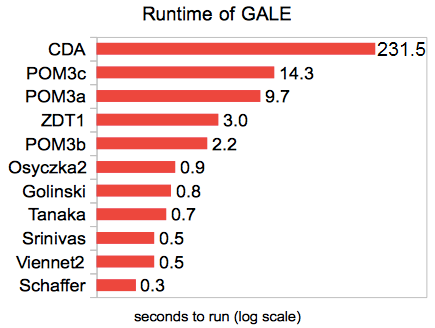
\includegraphics[width=2.75in]{figures/barcharts_runtime_galeAbsolute.png}
\caption{GALE, mean runtime in seconds.}\label{fig:runGale} 
\end{figure}






\begin{figure}[!h]
%\includegraphics[width=2in]{tim/runSpear2.png}\includegraphics[width=1in]{tim/runNsgaii.png}
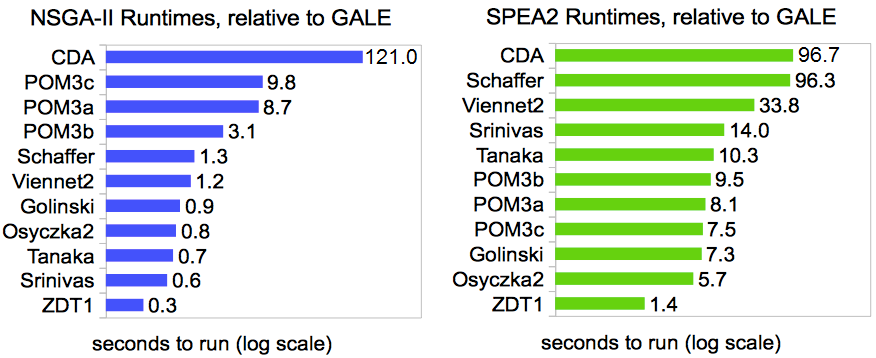
\includegraphics[width=3.49in]{figures/barcharts_runtime_relativeToGale.png}
\caption{NSGA-II, SPEA2, runtimes, relative to GALE (mean values
over all runs) e.g.,
with SPEA2, ZDT1 ran 1.4 times slower than GALE.}\label{fig:runSpea2} 
\end{figure}


\fig{runSpea2} compares GALE's runtimes to those
of NSGA-II and SPEA2. In that figure, anything with a relative
runtime over 1.0 ran {\em slower} than GALE. Note that 
GALE was faster than SPEA2 for all models. However,
for small models, GALE was a little slower than NSGA-II (by a few seconds).
For the POM3 models, GALE ran up to an order of magnitude faster than both NSGA-II and SPEA2.
As to CDA, GALE ran two orders of magnitude faster (terminating in 4 minutes versus 7 hours).



\fig{evals}  shows why GALE  runs so much faster than NSGA-II and SPEA2.
This figure shows the number of model evaluations.
Note that NSGA-II and SPEA2 needed between 1,000 and 4,000 evaluations for each model while GALE terminated after roughly 30 to 50 evaluations.
Across every model, SPEA2 and NSGA-II needed between 25 to 100 times more
evaluations to optimize (mean value: 55 times more evaluations).




\begin{figure}[!h]
%\includegraphics[width=3.5in]{tim/evals.png}
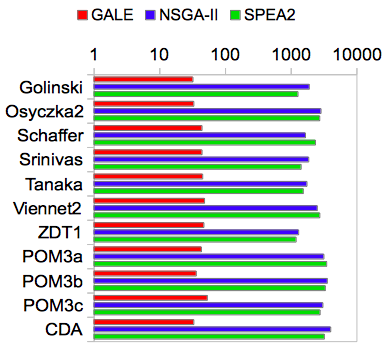
\includegraphics[width=2.75in]{figures/barcharts_numeval.png}
\caption{Number of evaluations (means over all runs), sorted
by  max. number of evaluations.}\label{fig:evals} 
\end{figure}


%% \begin{figure}[!t]
%% \begin{center}
%% \footnotesize
%% \begin{tabular}{|c@{~}|c@{~}|c@{~}|c@{~}|c@{~}|} \hline
%% Model      & NSGA-II       & GALE       & SPEA2       & Compared  \\ \hline \hline
%% Model      & NSGA-II       & GALE       & SPEA2       &  \\ \hline \hline
%% Golinski   & 1,890         & 32         & 1,270       & 49x     \\ \hline
%% Osyczka2   & 2,850         & 33         & 2,720       & 84x     \\ \hline
%% Schaffer   & 1,650         & 44         & 2,340       & 45x     \\ \hline
%% Srinivas   & 1,850         & 44         & 1,420       & 38x     \\ \hline
%% Tanaka     & 1,740         & 45         & 1,530       & 36x     \\ \hline
%% Viennet2   & 2,500         & 48         & 2,730       & 55x     \\ \hline
%% ZDT1       & 1,300         & 47         & 1,190       & 26x     \\ \hline \hline
%% POM3a      & 3,150         & 43         & 3,470       & 78x     \\ \hline
%% POM3b      & 3,550         & 36         & 3,310       & 95x     \\ \hline
%% POM3c      & 3,040         & 53         & 2,760       & 55x     \\ \hline \hline
%% Median     & 2,195         & 44         & 2,530       & 54x     \\ \hline
%% \end{tabular}
%% \end{center}
%% \caption{Number of Evaluations for each MOEA as averaged across all runs for that model.}
%% \label{fig:numeval}
%% \end{figure}


%% \begin{figure}[!t]
%% \begin{center}
%% \footnotesize
%% \begin{tabular}{|c@{~}|c@{~}|c@{~}|c@{~}|} \hline
%% Model      & NSGA-II     & GALE        & SPEA2 \\ \hline \hline
%% Golinski   & 0.7         & 0.8         & 5.8    \\ \hline
%% Osyczka2   & 0.7         & 0.9         & 5.1    \\ \hline
%% Schaffer   & 0.4         & 0.3         & 28.9   \\ \hline
%% Srinivas   & 0.3         & 0.5         & 7.0    \\ \hline
%% Tanaka     & 0.5         & 0.7         & 7.2    \\ \hline
%% Viennet2   & 0.6         & 0.5         & 16.9   \\ \hline
%% ZDT1       & 0.9         & 3.0         & 4.1    \\ \hline \hline
%% POM3a      & 84.7        & 9.7         & 78.4   \\ \hline
%% POM3b      & 6.8         & 2.2         & 20.8   \\ \hline
%% POM3c      & 140.5       & 14.3        & 107.2  \\ \hline \hline
%% Average    & 23.6        & 3.3         & 28.1   \\ \hline 
%% Median     & 0.7         & 0.9         & 12.1   \\ \hline
%% IQR        & 4.7         & 2.3         & 20.8   \\ \hline
%% \end{tabular}
%% \end{center}
%% \caption{CPU RunTime in seconds for each MOEA as averaged across all runs for that model.}
%% \label{fig:runtime}
%% \end{figure}

\subsection{Exploring RQ2 (Quality)}

The above results show GALE running faster than other MOEAs.
While this seems a useful result, it would be irrelevant if
the quality of the solutions found by GALE were much worse than other MOEAs.



\begin{figure}
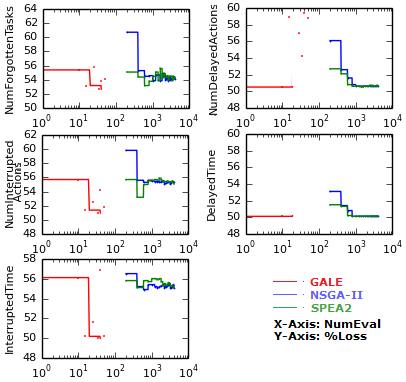
\includegraphics[width=3.3in]{figures/cda.png}
\caption{Execution traces of CDA. C-axis shows number
of evaluations (on a logarithmic scale). 
Solid, colored lines  show  best reductions seen
at each $x$ point.
The y-axis values show percentages of initial values
(so $y=50$ would mean {\em halving} the original value).
For all these
objectives, {\em lower} y-axis values are {\em better}.
}\label{fig:cda} 
\end{figure}

\begin{figure}
\begin{center}
\footnotesize
\begin{tabular}{lc@{~}|c@{~}|c@{~}|c@{~}} 
Type&Model      & NSGA-II      & GALE         & SPEA2 \\ \hline 
small&Golinski   & 76\%         & \colorbox{lightgray}{68\%}         & 74\%  \\ 
&Osyczka2   & 75\%         & \colorbox{lightgray}{72\%}         & 75\%  \\ 
&Schaffer   & \colorbox{lightgray}{62\%}         & 63\%         & \colorbox{lightgray}{62\%}  \\ 
&Srinivas   & 94\%         & \colorbox{lightgray}{84\%}         & 94\%  \\ 
&Tanaka     & 84\%         & \colorbox{lightgray}{75\%}         & 84\%  \\ 
&Viennet2   & \colorbox{lightgray}{73\%}         & 75\%         & \colorbox{lightgray}{73\%}  \\
&ZDT1       & 87\%         & \colorbox{lightgray}{80\%}         & \colorbox{lightgray}{82\%}  \\ \hline 
medium &POM3a      & 92\%         & 91\%         & \colorbox{lightgray}{90\%}  \\
&POM3b      & 91\%         & \colorbox{lightgray}{90\%}         & \colorbox{lightgray}{90\%}  \\ 
&POM3c      & 93\%         & 90\%         & 93\% 
\end{tabular}
\end{center}
\caption{Median scores comparing final frontier values
to initial populations. Calculated using \eq{cdom}.
{\em Lower} scores are {\em better}.
Gray cells are significantly
different (statistically) and better than the other values in that row.}
\label{fig:scores}
\end{figure}



\begin{figure*}[!t]
%\centering
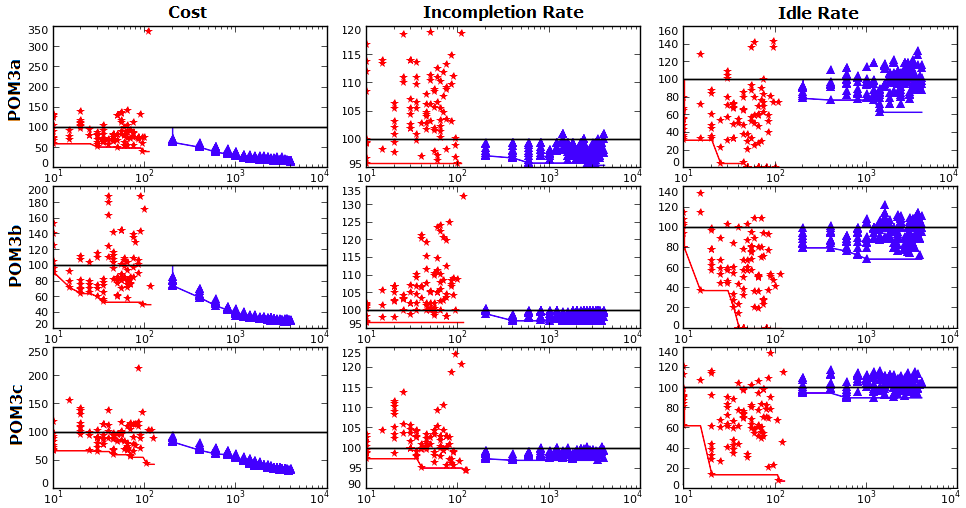
\includegraphics[width=6.8in]{figures/figure_analytics_obj_score_plots.png}
\caption{POM results: 20 repeats of each MOEA (one row
per scenario) from
\textcolor{red}{{\bf GALE (red)}}
and 
 \textcolor{blue}{{\bf NSGA-II (blue)}}. Each y-axis represents the percent objective value relative
to that in the initial baseline population, and lower is better.
The lines trend across the best (lowest) seen objective thus far.  Each x-axis shows number of evaluations (log scale. }
\label{fig:zdt1objspace}
\end{figure*}



One issue with exploring solution quality
with the CDA model was that NSGA-II and SPEA2 ran so slow that 20 runs would 
require nearly an entire week of CPU.
Hence, in this study NSGA-II and SPEA2 were
only run once on CDA.  \fig{cda} shows those results.
Note that GALE achieved the same (or better) minimizations, using  fewer evaluations than NSGA-II or SPEA2. 


As to the other models,
to summarize the improvements in solution quality, we report how much
the score (``loss'' from \eq{cdom}) changes from the initial population to the final frontier
returned by each MOEA.  Recall from~\tion{cdom} that this measure summarizes the
improvement over all objectives.

\fig{scores} shows these change values,
as seen in 20 repeated runs of the models. 
For that figure, {\em lower} scores are {\em better}.
In that figure, the cells shown in gray in \fig{scores}
are the values
that are statistically best (this test was applied across
all the values in each row using a Mann-Whitney 99\% confidence procedure).
Measured in terms of number of wins (the gray cells), GALE wins more
than the other MOEAs. Also, when it is not the best in each row,
it loses by very small amounts (never more than 3\%).







An issue with summary statistics
like \fig{scores}  is that such summaries can hide significant effects.
For example, all the \fig{scores} results from POM3 are very close to 90\%
suggesting that, for this model, all MOEAs produced similar
results.
Yet a closer inspection of those results shows that this is not the case.
\fig{zdt1objspace} shows how NSGA-II and GALE evolved candidates
with better objective scores.  
The y-vertical-axis denotes
changes from the median of the initial population.
 That is:
\bi
\item $Y=50$ would indicate that we have halved the value of some objective;
\item $Y \gt 100$ (over the solid black line) would indicate that optimization failed to improve this objective.
\ei
In \fig{zdt1objspace}, all 
the y-axis values are computed such that {\em lower}
values are {\em better}. Specifically, the results in the column
labeled {\em Incompletion Rate}
is the ratio {\em initial/now} values. Hence, if we are {\em now} completing a larger
percentage of the requirements, then {\em incompletion} is better if it is
less than 100\%; i.e. \[\mathit{Incompletion}\% = 100 - \mathit{Completion}\%\]
At first glance, these results seem to say that GALE
performed worse than NSGA-II since NSGA-II achieved larger
{\em Cost} reductions. However, the {\em Idle}
results  show otherwise:
 NSGA-II rarely reduced
the {\em Idle} time of the developers  while GALE
found ways to achieve reductions down to bear zero percent {\em Idle}.

This observation begs the question: how could
NSGA-II reduce cost while increasing developer {\em
  Idle} time?   One answer is some quirk in the input space.
However, that answer is not supported; observe that the same strange pattern
(of increased {\em Idle} and decreased {\em Cost}) holds
in POM3a and POM3b and POM3c).

A better explanation can be found in the  {\em Incompletion Rate}
results: NSGA-II told the developers to complete
fewer requirements. Since POM3 measures cost in
terms of the {\em salary times effort} for the
completed requirements, then by completing fewer
requirements, NSGA-II could reduce the reported cost.
Note that this is not necessarily an error in the  POM3 costing routines- providing that an optimizer
also avoids leaving programmers idle.
In this regard, NSGA-II is far worse than GALE since the latter
successfully reduces {\em cost} as well as the {\em Idle Rate}.

We conjecture that NSGA-II's failure in this regard
was due to its use of a binary dominance function. As discussed in \tion{cdom},
continuous domination functions, such as that used by GALE, can find more
nuances in the trade-offs between competing objectives.
In support of this conjecture, we note that SPEA2, which also uses binary domination,
also suffers from large {\em Idle Rates} in the final frontier of POM3 outputs\footnote{
Those SPEA2
results look very similar to the NSGA-II results of  \fig{zdt1objspace}.
Those results are not shown here due to space reasons.}.



\subsection{Answers to Research Questions}

{\bf RQ1 (speed):} {\em Does GALE terminate faster than other SBSE tools?}:

Note that 
for  smaller models, GALE was slightly slower than NSGA-II (but much faster than SPEA2).
Also, for large models like CDA, GALE was much faster.
These two effects result from the relative complexity
of (a)~model evaluation versus (b)~GALE's internal clustering of the data.
When model evaluation is very fast, the extra time needed for clustering
dominates the runtimes of GALE.  However, when the
model evaluation is very long, the time
needed for GALE's clustering is dwarfed by the evaluation costs. Hence,
GALE is strongly recommended for models that require long execution times.
Also, even though is slower for smaller models, we would still  recommend for those
small models.
The delta between absolute runtimes of GALE and the other optimizers is negligible ($\le 3$ seconds).
Further, GALE requires fewer evaluations thus reducing the complexity
for anyone working to understand the reasoning (e.g.  a
programmer conducting system tests on a new model).

{\bf RQ2 (quality):} {\em Does  GALE  return  similar or better solutions than other SBSE tools?}:

GALE's solutions are rarely worse than other optimizers (and sometimes, they are 
better).


\section{Threats to Validity}

As with any empirical study, biases can affect the
final results. Therefore, any conclusions made from
this work must be considered with the following
issues in mind.

\subsection{ Sampling Bias}
This bias threatens any conclusion based on the
analysis of a finite number of optimization
problems.  Hence, even though GALE runs well on
the models studied here, there may well be other
models that could defeat GALE.  

For this issue of sampling bias, the best we can do
is define our methods and publicize our tools so
that other researchers can try to repeat our results
and, perhaps, point out a previously unknown bias in
our analysis. Hence, all the experiments (except for
CDA) in this paper are available as part of the JMOO
package that contains GALE (see
http://unbox.org/open/tags/JMOO).  Hopefully, other
researchers will emulate our methods to repeat,
refute, or improve our results.

\subsection{Optimizer Bias}
Another source of bias in this
study are the optimizers (MOEAS) used for comparison purposes.
Optimization is a large and active field
and any single study can only use a small subset of
the known optimization algorithms. In this work,
only results for GALE, NSGA-II and SPEA2 are published. Our reasons for selecting
these last two were cited above: based on a recent survey of SBSE tools~\cite{sayyad13c}, it is clear
that these tools are currently the most commonly used in this field.

\subsection{Parameter Bias}


For this study, we did not do extensive parameter tuning:
NSGA-II and SPEA2 were run using their default settings
while GALE was run using the settings that worked well on the first model  we
studied (the Schaffer model of \fig{nocon}) which were then frozen for the
rest of this study. As documented above, those parameters were:
\bi
\item $\mu$ = 100:  population size;
\item $\omega$ = $\sqrt{\mu}$: minimum size leaf clusters;
\item $\lambda = 3$: premature stopping criteria (sets the
maximum allowed 
generations without
any improvement on any objective).
\ei
If this paper was arguing that these parameters were somehow {\em optimal},
then it would be required to present experiments defending the above settings.
However, our  claim is less than that- we only aim  to show
that with these settings, GALE does as well than standard
SBSE tools. In future work, we will explore other  settings.

\subsection{Evaluation Bias}
This paper has evaluated MOEAs on runtimes,
number of evaluations,
and solution quality. The latter was assessed
using changes in the \eq{cdom} score (assessed via a Mann-Whitney
test) as well as the visualizations of \fig{cda}
and \fig{zdt1objspace}.






Alternate measures for assessing MOEAs are the
{\em GD}
{\em generational distance}, 
the {\em HV} hypervolume;
and
the {\em spread} of solutions over the Pareto frontier.
As to the {\em spread} measure, this scores high if
many solutions are well-spaced across the Pareto
frontier. Spread can be inappropriate for the
solutions returned by GALE since the distance
between GALE's solutions on the frontier are
selected by a user-supplied parameter (the {\em
enough}) variable of \fig{galeCode}).  Hence, it can
be better to study GALE's spread visually, rather
than rely of the standard algebraic definitions of
spread.  For example \fig{golspread} shows GALE's
final frontier found using a very small value to
{\em enough}. Also shown in that figure are the
initial population and the frontier found by NSGA-II
and SPEA2.  

\begin{figure}[!b]
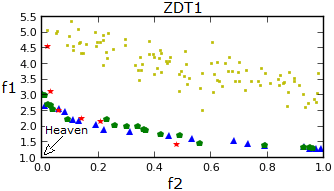
\includegraphics[width=3.49in]{figures/figure_analytics_objective_space.png}
\caption{Final frontiers found by 
\textcolor{blue}{{\bf NSGA-II} (blue)}, \textcolor{darkgreen}{{\bf SPEA2} (green)}, and \textcolor{red}{{\bf GALE} (red)} on ZDT1 (minimizing both objectives).  Yellow markers show the initial population.}\label{fig:golspread}
\end{figure}


Note that, by design, GALE finds fewer
examples on the frontier than other MOEAs (and
this can be changed by altering the {\em enough}
parameter).  Note also that NGSA-II and
SPEA2 have ``better'' spreads in the $x$ direction (SPEA2 and 
NSGA-II's solutions extend beyond those of GALE); but
in the $y$ direction, it is GALE that extends further.
This result is typical of other
results seen with GALE, NGSA-II and SPEA2; i.e.
reflecting on the final spread is not informative
for the purposes of ranking these MOEAs.



\begin{figure}[!t]

\begin{tabular}{|p{.95\linewidth}|}\hline
\small
GD
 reports the distance of the best instances
found by the MOEA to their nearest neighbor on the optimal Pareto frontier as
defined by Van Veldhuizen and Lamont~\cite{Veldhuizen98evolutionarycomputation}.
HV reports the size of the convex hull around the generated
solutions (including some reference points that include objective scores of zero), as
first sourced in literature in~\cite{Zitzler98multiobjectiveoptimization}.

For complex models, the location of the optimal Pareto frontier may not be known or computable
(and it is needed for GD and HV).
Also, 
if a  random placement of instances
can easily generate a large hypervolume, then large 
HV measures are no real measure of accomplishment
of the MOEA.
Further, GD gives preferential scoring to
Pareto frontiers of certain shapes- which may be an incorrect
assumption for certain models.
For example, Zitzler et al. \cite{Zitzler98multiobjectiveoptimization}
and Lizarraga et al.~\cite{Lizarraga-Lizarraga:2008:GMQ:1389095.1389227}
caution that 
GD
favors concavity of the Pareto frontier,
since, as typically defined,
it  biases towards external faces of convex
curves.

Lastly, measuring HV is not an easy task. It can be very cpu-intensive to calculate~\cite{bader11}
(formally it is P-Hard to
compute~\cite{Bringmann2010601}).  Also, the placement of the reference points used in HV is the
subject of questioning, as improper placement can lead to bias towards an extreme of the solution space.  
Typically the nadir point is used as the reference point (all objectives at worse score). 
The problem of appropriate placement of the reference point has been discussed
in~\cite{Auger:2009:THI:1527125.1527138}, so as to retain information about both extremes.   \\\hline
\end{tabular}
\caption{Issues with the GD and HV measures.}\label{fig:issues}
\end{figure}



As to other measures, as discussed in \fig{issues},
there are numerous technical issues associated with 
GD and HV. 
Apart from the issues of that figure, we have
methodological reasons for using \eq{cdom}
to compare our final frontier with the initial population.
Shepperd \& MacDonnell~\cite{shepperd12z} argue that 
performance results should be compared to
some stochastically selected baseline (which we do---using the items in
the initial population). 
GD and HV, on the other hand, have no ``zero'' value
against which we can judge any perceived improvement.



   
\section{Conclusions}
This paper has introduced GALE, an evolutionary
algorithm that combines active learning with
continuous domination functions and fast spectral
learning to find a response surface model; i.e. a
set of approximations to the Pareto frontier.
We showed that for a range of scenarios and models
that GALE found solutions equivalent or better than
standard methods (NSGA-II and SPEA2).  Also, those
solutions were found using one to two orders of
magnitude fewer evaluations.

We claim that GALE’s superior performance is due to
its better understanding of the shape of Pareto
frontier.  Standard MOEA tools generate too many
solutions since they explore uninformative parts of
the solution space.  GALE, on the other hand, can
faster find best solutions across that space since
it understands and exploits the shape of the Pareto
frontier.


These results suggest that it is perhaps time to reconsider the random
mutation policy used by most MOEAs.  GALE can navigate the space of
options using far fewer evaluations that the random mutations of
NSGA-II and SPEA2. We would propose a ``look before you leap'' policy;
i.e. before applying some MOEA like SPEA2 or NSGA-II, cluster the
known solutions and look for mutation directions in the non-dominated
clusters.

   

\section{Acknowledgements}

The work was funded by NSF grant CCF:1017330 and the
Qatar/West Virginia University research grant NPRP
09-12-5-2-470.  This research was partially
conducted at NASA Ames Research Center. Reference
herein to any specific commercial product, process,
or service by trade name, trademark, manufacturer,
or otherwise, does not constitute or imply its endorsement by the United States Government.

\bibliographystyle{IEEEtran}

\bibliography{references}%,efstim}

    
    %\underline{{\bf FINAL SCORING:}}
    %The POM models score a planning policy by comparing a developers' {\em %incremental} decisions
    %to those that might have been made by some omniscient developer (that has access
    %to the   {\em final} cost and priority of requirements).


 

\begin{IEEEbiography}[{
\includegraphics[width=1in,clip,keepaspectratio]{images/joe.jpg}} ]{Joseph Krall}
is a Ph.D. student at West Virginia University, studying Computer Science with research interests in Games Studies, Cognitive \& Psychological Sciences in Gaming, Artificial Intelligence, Data Mining, and Search Based Software Engineering.  Joseph (Joe) has received a B.S. in Computer Science and Mathematics at the University of Pitt-Johnstown (2008), and  M.S. in Computer Science at West Virginia University (2010).
\end{IEEEbiography}

\begin{IEEEbiography}[{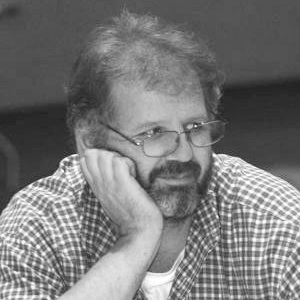
\includegraphics[width=1in,clip,keepaspectratio]{images/timm.jpg}}]{Tim Menzies} (Ph.D., UNSW)
is a Professor in CS at WVU and  the author of
over 200 referred publications. In terms of citations, he is one of the top 100 most
most cited
authors in  software engineering (out of 54,000+ researchers, see
http://goo.gl/vggy1). At WVU, he has been a lead researcher on
projects for NSF, NIJ, DoD, NASA, as well as joint research work with
private companies. He teaches data mining and artificial intelligence
and programming languages. Prof. Menzies is the co-founder of the
PROMISE conference series (along with Jelber Sayyad) devoted to reproducible experiments in
software engineering: see http://promisedata.googlecode.com. He is an
associate editor of IEEE Transactions on Software Engineering. the Empirical Software Engineering Journal, and the
Automated Software Engineering Journal.  For more information, see his web site http://menzies.us
or his vita at http://goo.gl/8eNhY or his list of publications at
http://goo.gl/8KPKA .
\end{IEEEbiography}


\begin{IEEEbiography}[{
\includegraphics[width=1in,clip,keepaspectratio]{images/davies1_gs.jpg}}]{Misty Davies}
(Ph.D. Stanford),is a Computer Research Engineer at
  NASA Ames Research Center, working within the
  Robust Software Engineering Technical Area.  Her
  work focuses on predicting the behavior of
  complex, engineered systems early in design as a
  way to improve their safety, reliability,
  performance, and cost. Her approach combines
  nascent ideas within systems theory and within the
  mathematics of multi-scale physics modeling.
For more information, see her web site http://ti.arc.nasa.gov/profile/mdavies
or her  list of publications at
http://ti.arc.nasa.gov/profile/mdavies/papers.
\end{IEEEbiography}

\clearpage
 \setcounter{page}{1}
\pagenumbering{Roman}
\section*{Reply to Reviewers}
\subsection*{Comments from the Associate Editor}

Dear Prof. Cleland-Huang, 

Please thank your reviewers for their excellent review notes from our
prior draft. 
Using that feedback, we  have extensively revised the prior draft which
we now submit for your consideration. 

In the notes below, we detail how this draft differs from the first one. Note that paragraphs in {\bf {\em bold italics}}
are text taken from the prior review.


You write: {\bf {\em Based on the reviewers comments I am unable to
  recommend this paper for TSE.  The recurring theme
  in the reviewers comments (both public and
  private) is that the paper is poorly written and
  therefore hard to understand.}}
  
 

We concur.  This new paper is built around a structure proposed by Reviewer2 and
Reviewer3 who both said that the core issues of this paper are:
\bi
\item
{\bf RQ1 (speed):} Does GALE terminate faster than other SBSE tools?
\item 
{\bf RQ2 (quality):} Does GALE return  similar, or better,
solutions than other SBSE tools?
\ei
Please note that we now list these questions in the introduction and that our
new results section is based on these two questions.

As to the half dozen research questions in the last draft, 
we have replaced them with the above two.

We have also improved the last draft with structural features
and have added much more detail  in order
to improve its comprehensibility:
\be
\item We offer a (very) abridged summary of the new algorithm, on page 2;
\item We added extensive notes on the background of search-based SE on page 2, page 3;
\item We offered detailed pseudo-code of the new algorithm on page 4, page 5, page 6;
\item We rewrote the results section on page 9, page 10, page 11 to greatly simplify the results section.
\item  We added exact details on the algorithm's pseudocode on page 4, page 5, and page 6.
\ee

You also write: {\bf {\em It lacks sufficient details of the
    approach.  One reviewer (\#1) has more serious
    issues with (a)~the scope of the paper and
    (b)~the delta of the contribution above and
    beyond prior work.}}


We completely agree that the last draft of the paper had the
wrong scope: it should have been more about the GALE
algorithm and less about the agile model.  That has been fixed in this draft (using the excellent 
suggestions from the last round of review regarding the two core research questions, shown above).

We further agree that  the new version of POM3 is not unique or interesting
enough  to justify journal publication at TSE.  Instead, this paper is about
 a new search-based SE algorithm
that runs orders of a magnitude faster than the
state-of-the-art.

Also, to increase the delta from prior work, we have 
added a completely new case study (the NASA human-automation cockpit model called CDA- see page 8, page 9).



\subsection*{Reviewer 1}


{\bf {\em The authors build upon the previously published
  POM1 and POM2 models and propose GALE to improve
  the performance of POM3 (specifically, to reduce
  the number of evaluations that are needed). The
  authors base the experiments on four scenarios and
  show that the proposed method achieves results
  that are comparable to other methods (e.g.,
  NSGAII) but with fewer number of model
  evaluations.  One major problem of the current
  manuscript is that how much contribution POM3
  makes.}}

We very much agree with you.  In this draft, the contribution of this paper is the GALE algorithm.

As to the POM3 model of agile development, that is now merely just one of the eight models studied in this paper.
Using those models we make the case that our ``geometric active learner'' can find competitive solutions for SBSE problems,
using 10 to 100 times fewer evaluations than established practice.


{\bf {\em Another major drawback relates to the four
  scenarios that the author used to evaluate
  GALE. The choices were made without any
  explanation and justification -- except that "it
  is an interesting subset". However, many other
  scenarios may be equally "interesting" and POM3d
  (small, seldom changing projects) does *NOT* seem
  to belong to agile development's scope of
  applicability and therefore is *NOT*
  interesting. }}

We completely agree- especially about POM3d (which
has been excluded from this draft).

As to why we still use the other POM3 scenarios; it
turns out that there was an interesting meta-level
issue with how the other MOEAs handled the POM3
model. When exploring that issue, we found it useful to
run three different input scenarios (in order to
verify that the issue was not a quirk of some
input). We now say at end of section 4.2.2 that:
\begin{quote}
When we ran POM3 through various MOEAs, we noticed a strange pattern in the results
(discussed below). To check if that pattern was a function of the model or the MOEAs,
we ran POM3 for the three different kinds of projects shown in \fig{pom3decisions}.
We make no claim that these three classes represent the space of all possible projects.
Rather, we just comment that for more than one class of agile projects,
GALE appears to out-perform NSGA-II and SPEA2.
\end{quote}
 But apart from that, we acknowledge your point
 that these scenarios do not reflect the
 space of all possible agile projects, and merely that
 GALE can work for the scenarios (arbitrarily) selected.

{\bf {\em  A significant flaw in formulating research
    questions appears between RQ3 and RQ4. The
    authors have presumed the answer to RQ1-RQ3 is
    "yes". A more empirically rigorous way is to
    formulate null hypothesis and formulate further
    hypothesis based on the *actual* statistical
    test results.}}

We agree that the research questions in the prior draft were poorly formed. We do not reuse them here.  Instead, we base this
paper on two core issues identified by reviewers in the last round:
\bi
\item
{\bf RQ1 (speed):} Does GALE terminate faster than other SBSE tools?
\item 
{\bf RQ2 (quality):} Does GALE return  similar, or better,
solutions than other SBSE tools?
\ei
Please note that we now list these questions in the introduction and that our
new results section is based on these two questions.
As to the half dozen research questions in the last draft, there were confused and
we have replaced them with the above two.


{\bf {\em
Overall the paper is well-written. A few grammar-related errors are listed as follows.
(omitted for simplicity and space).}}

We thank you for these corrections.  Note however that after a revision, many of these
have gone away and otherwise have been corrected.

\subsection*{Reviewer: 2}

(Please note that Reviewer2 listed several typos and minor editorial issues
that have been addressed in this draft.)

To begin our reply to your comments, we wish to start with one of your latter points:

{\bf {\em There are basically two fundamental questions regarding GALE, a first concerning the number of evaluation compared to that of other algorithms and a second concerning the quality of the results it returns (does it find roughly the same solutions as other algorithms?).}}

You are correct. Your proposed sequence is now the overall guiding
principle of this paper- see page2, page9, page10, page11.

Returning now to the start of your comments...

{\bf {\em The results claimed by this paper are
    impressive: if true, it would be a major
    breakthrough in MOEA with high impacts both in
    search-based software engineering and
    multi-objective optimisation in general. }}

Thank you for that comment.

{\bf {\em This result is however hard to validate because the presentation is inadequate.
In Section 4, the new MOEA algorithm is not described clearly enough to allow
other researches to understand and implement it. The algorithm is actually never
shown in full. (Section 4.1, called "Details", give details about the validation
experiment rather than details of the algorithm; this information should be moved
to the experiment section.)}}

We agree- this draft  now has 
\be
\item A high-level summary of the new algorithm, page2;
\item Detailed pseudo-code of the new algorithm on page4, page5, page6.
\ee

{\bf {\em
The POM3 model, which is said to be presented in this paper for the first time, is 
presented only very summarily. There is not enough information to understand the model, 
what decisions it supports (Fig. 4 is not enough; it needs explanations), and why its 
three objectives are valid (I'm surprised by the objective to minimise idle rate which 
appears to contradict a fundamental principle of lean development which is to maximise 
value creation instead of resource utilisation).}}

We agree that there was too much POM3 in the last version- now it is just one of the eight models
explored to test the new algorithm.

As to your specific point (that POM3 should be about resource utilization) please note: that
is actually in the current version of POM3. Requirements development cost is measured using programmer
salaries. We also have an {\em Idle rate} measure which we need to minimize. So the current goals
of POM3 are to make the most use of the programmer's busy time (when working on some current requirement)
while minimizing their wasted time (measured as the {\em Idle Rate} when they are forced to wait
on the delivery of other requirements).


{\bf {\em It is actually not clear why POM3 is presented in the paper. If the paper's core contribution is GALE, wouldn't it be simpler and better to demonstrate GALE's benefits on previously published models in search-based software engineering? One of the difficulties in reading the paper is that it mixes two novel contributions, GALE and POM3, without clearly distinguishing them, neither in their presentation nor in the experiments. Maybe this work needs to be split in two separate papers, one about GALE and one about POM3, each describing and validating its contribution in full details.}}

We agree- and this draft was written as per your direction. This paper is now mostly about certifying
the GALE algorithm (via a comparative assessment with rival algorithms).

{\bf {\em The validation section (Section 6) does not present the results clearly.  Given the strong claims in introduction, one would expect a clear and direct comparison of GALE with respect to other MOEA on a set of problems. }}

We completely agree. The results section of the last draft has been significantly rewritten and simplified.
As to the research questions of the last draft, they were poorly formed and so are not used in this draft.



{\bf {\em The paper's arguments why it is important to reduce the number of evaluations performed by a MOEA are weak and partly incorrect (Section 2).}}

We agree- we have now dropped all of that material in this draft.


{\bf {\em The claimed improvements of GALE over NSGA-II and
other MOEAs is very impressive. Often such
improvements are only possible by compromising
something but I could not identify whether or what
compromises are being made in this case. Are there
limitations to the use of GALE over NSGA-II and other
MOEAs? Do we lose something by using GALE instead of
NSGA-II? }}

In response to this question, we have tried many
tests- even printing out and manually inspecting all
the Pareto frontiers generated by all these
MOEAs on all these models (for one sample of
that print out, please see the last figure in the
paper).

To date, we have not found some compelling reason not to use GALE- which is not to say that the
model we use tomorrow might raise novel issues that would mean we have to revise our optimism for
this new algorithm (a point that we stress in the ``Threats to Validity'' 
section on p11).



\subsection*{Reviewer: 3}

(Please note that Reviewer3 listed several typos and minor editorial issues
that have been addressed in this draft.)

To begin our reply to your comments, we wish to start with one of
your latter points:

{\bf {\em What I am really missing (and should I had
    found it in the paper, I would have recommended
    a no-doubt accept) is a replication package,
    with the implementation of the algorithms, and a
    dataset to test the different algorithms,
    possibly with suggestions and guidelines about
    how to apply GALE with other models (for
    instance, elaborating more on what "engineering
    judgment" is necessary to adapt GALE to other
    models). }}

That replication package is now available on the web (see Section 1.2 on page2).
That replication package comes with most
of this study's  models  (sadly, the CDA
model is a specialized NASA product that we cannot
release to the public).

As to how to apply GALE to different models, please
see the start of section 3 (top left of page5)
listing the ``glue'' functions that connect GALE to
a model.

Returning now to the start of your comments...

{\bf {\em This paper presents a multi-objective
    optimization algorithm for software projects,
    called GALE. It is tested with the POM3 model,
    providing results that could be useful for the
    management of software agile projects. GALE is
    compared with other algorithms to assess that it
    requires less iterations to obtain a result.

The paper presents the following points in favor and against, that we will comment with more detail below:

Pros: (1)~New algorithm more suitable for software engineering than other alternatives;
(2)~Tested with a model that seems to be a "real world" example
(3)~Example of application of the algorithm included in the paper
}}

Thank you for your kind words. Please note that this draft now has case studies on {\em two} real world
models (POM3 and the NASA CDA model on avionics safety).

{\bf {\em Cons: Research questions are more focused in the POM model than in the algorithm}}


We agree. Those research questions were poorly defined and are not reused here. Instead,
we follow the advice of Reviewer2 who wrote 
``There are basically two fundamental questions regarding GALE, a first concerning the number of evaluation compared to that of other algorithms and a second concerning the quality of the results it returns (does it find roughly the same solutions as other algorithms?''. Accordingly, 
those two fundamental questions are addressed
in this paper- see page2, page9, page10, page11.

{\bf {\em  Not clear whether the decisions made by GALE are better or worse (or none) than those suggested by other algorithms:}}

This is our new RQ2 (quality).  We think Figures 17,18,19 show that GALE's
decisions can be better than those found by other algorithms.


{\bf {\em 
As described in section 3.4, GALE has seven tuning parameters that must be set in order to apply the algorithm. However, in section 5, when GALE is assessed, not all these parameters are set. In particular, where is the delta parameter? }}

We were certainly guilty of over-specification in the last draft. GALE has been significantly
simplified for this new draft and now it uses just the three tuning parameters listed in Section 6.3


{\bf {\em GALE is already difficult to understand, and this mismatch has left me puzzled wondering how GALE is supposed to be used.}}

You are correct- our previous description was far too complicated.
This draft  now has 
\be
\item A high-level summary of GALE, page2;
\item Detailed pseudo-code of the new algorithm on page4, page5, page6.
\ee


{\bf {\em Moreover, these tuning parameters are not
    explained with enough detail. It is not clear
    how these parameters must be chosen. The authors
    just say that they selected using their
    "engineering judgement", but I think that is
    very vague to say so. After all, you are
    comparing against other methods. How do I know
    that you have not tweaked the parameters to
    perform better in this particular setting? (with
    this model, against the other particular
    algorithms) How do I know that the better
    performance will hold in other scenarios?}}

You raise two important questions:
\bi
\item In section 6.3, we note
that we froze GALE's tuning parameters after some exploration of the smallest model (and that we did
so before starting our work on NSGA-II and SPEA2).
\item As to your other question (will these work for all scenarios), as we say in Section 6.1,
there is no general answer to that issue. Hopefully, now that our replication package is on-line,
we can work with other researchers to define some context space within which we'd recommend
GALE, and outside of which we would not.
\ei

{\bf {\em Now I would like to comment on the
    research questions posed in the paper. There are
    seven research questions and some of them seem
    to be very focused on POM3 as a model for
    software projects, rather than on the features
    of GALE compared against other MOEAs. I can
    extract one very clear conclusion out of those
    questions: GALE is faster. I grant you that. But
    it is not clear at all how the quality of the
    decisions made by GALE is compared against the
    decisions made by the other algorithms.}}

Those research questions were ill-formed and we do not reuse them here.
Instead, we use the research questions based on your comments (see the research
questions {\bf RQ1} and {\bf RQ2} defined on page2 and discussed on 
page9, page10, page11.

As to the comparative quality of GALE's solutions w.r.t. other models,
as mentioned above, we believe Figures 17,18,19 show that GALE's
decisions can be better than those found by other algorithms. But, what is your view?


{\bf {\em Because all of these three points (how to apply GALE?
what's the impact on decisions of the algorithm compared to existing options?
the lack of replication package and application guidelines), I recommend a major revision.}}

Please advise: has this draft addressed the matters you raised here?


\end{document}

We quickly concluded that these models are poorly suited to conventional optimization methods.
In order to speed up those simulations, we analyzed the CDA model with GALE.  

The model is a hybrid system and is governed both by continuous dynamics (the physics that allows flight) and also discrete events (the controllers' choices and aircraft modes)~\cite{Pritchett2001}.  
Such hybrid models are hard to analyze using classical optimization techniques that assume a model is Lipschitz continuous everywhere (i.e. has a smooth response surface). 
For smooth surfaces, it is possible to find a response surface that is arbitrarily close to our desired function using polynomial approximations by the Weierstrass Approximation Theorem~\cite{Bartle1976}. 
For the CDA model, no such guarantee of smoothness exists.  
Hence, the exploration of modal variables like the cognitive control mode usually requires combinatorial approaches such as GALE.
